\chapter{Sistema Final}

El sistema final es la culminación de los sistemas desarrollados en este proyecto, el cual parte del planteado para el sistema medio agregando funcionalidades extras al sistema que se detallarán más adelante. El mismo se encuentra planteado de manera que presente retrocompatibilidad, es decir, que todo software diseñado tanto para el sistema mínimo como para el sistema medio, debe funcionar en el sistema final. En comparación al sistema medio, se presentan la integración de la fuente de alimentación al sistema, el uso de memorias seriales, sistema de conversión AD, una interfaz de entrada salida expandida y un sistema de comunicación SPI.   
El circuito del sistema se encuentra diseñado, se presenta el esquemático, lista de componentes y diseño de placa PCB. No obstante, al momento de la escritura de este informe, el mismo no ha sido construido.

\section{Esquemáticos}
\label{C:EsqSF}
A modo de simplificar el análisis y presentación del sistema, el esquemático del mismo se presenta de manera modular, comenzando con el esquema generalizado (Ver figura \ref{F:EsquemaSF}) en el cual se pueden ver todas las partes que componen al sistema, sin adentrarse en un funcionamiento específico, para luego en las siguientes secciones pasar a especificar su funcionamiento.
Principalmente en este esquema podemos observar la interconexión entre el microprocesador y los dispositivos o periféricos asociados.

\begin{figure}[ht]
  \centering
  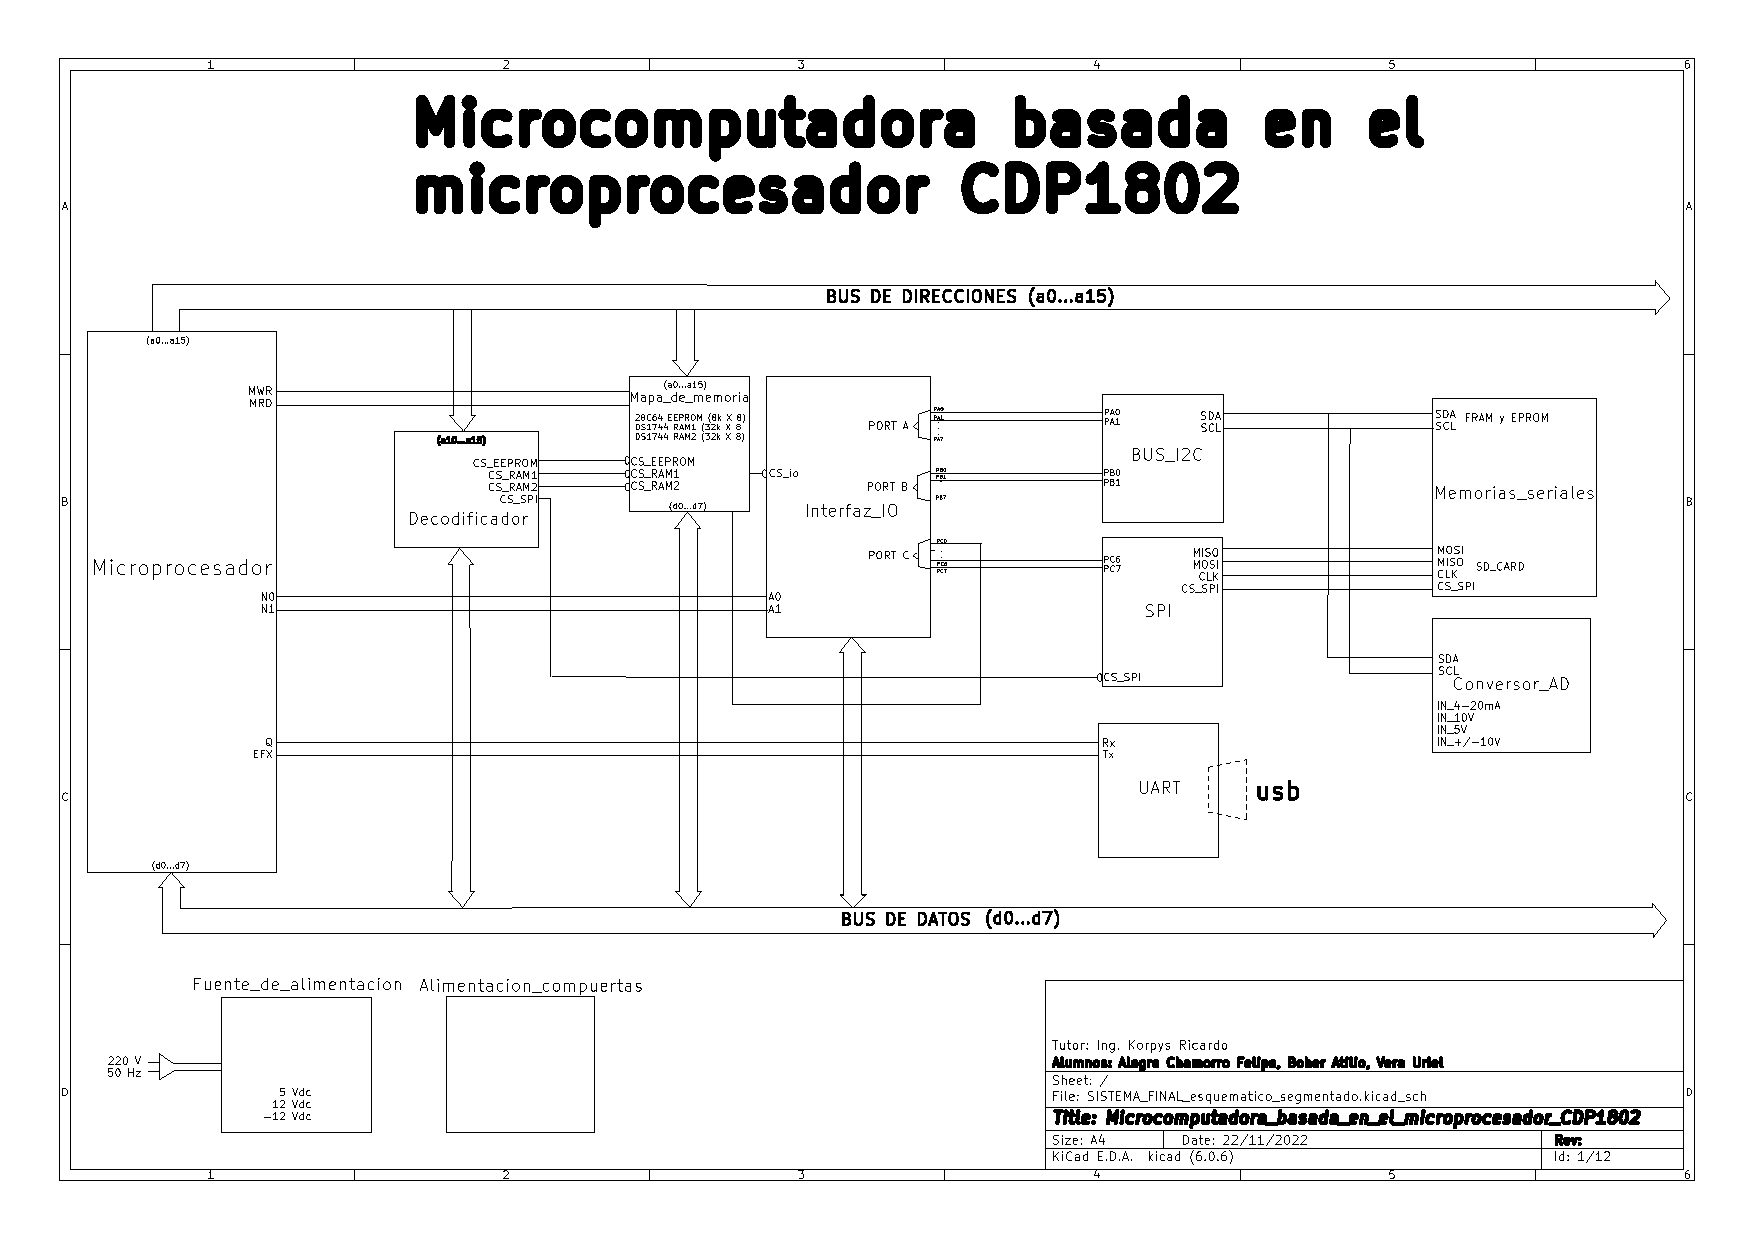
\includegraphics[width=1.2\textwidth, angle=90]{./imagenes/EsquematicosSF/Esquematico (1).pdf}
  \caption{Esquema general de sistema final}
  \label{F:EsquemaSF}
\end{figure}

\clearpage
\subsection{Fuente de alimentación}
La fuente de alimentación utilizada es lineal, basada en un transformador de tensión con punto medio. Dispone de un filtro de línea lo que reduce la distorsión armónica introducida en la red. 
Luego del proceso de rectificación y filtrado, se colocan etapas de regulación de tensión, para así poder alimentar los diferentes elementos del circuito que lo requieran. 

\begin{figure}[ht]
  \centering
  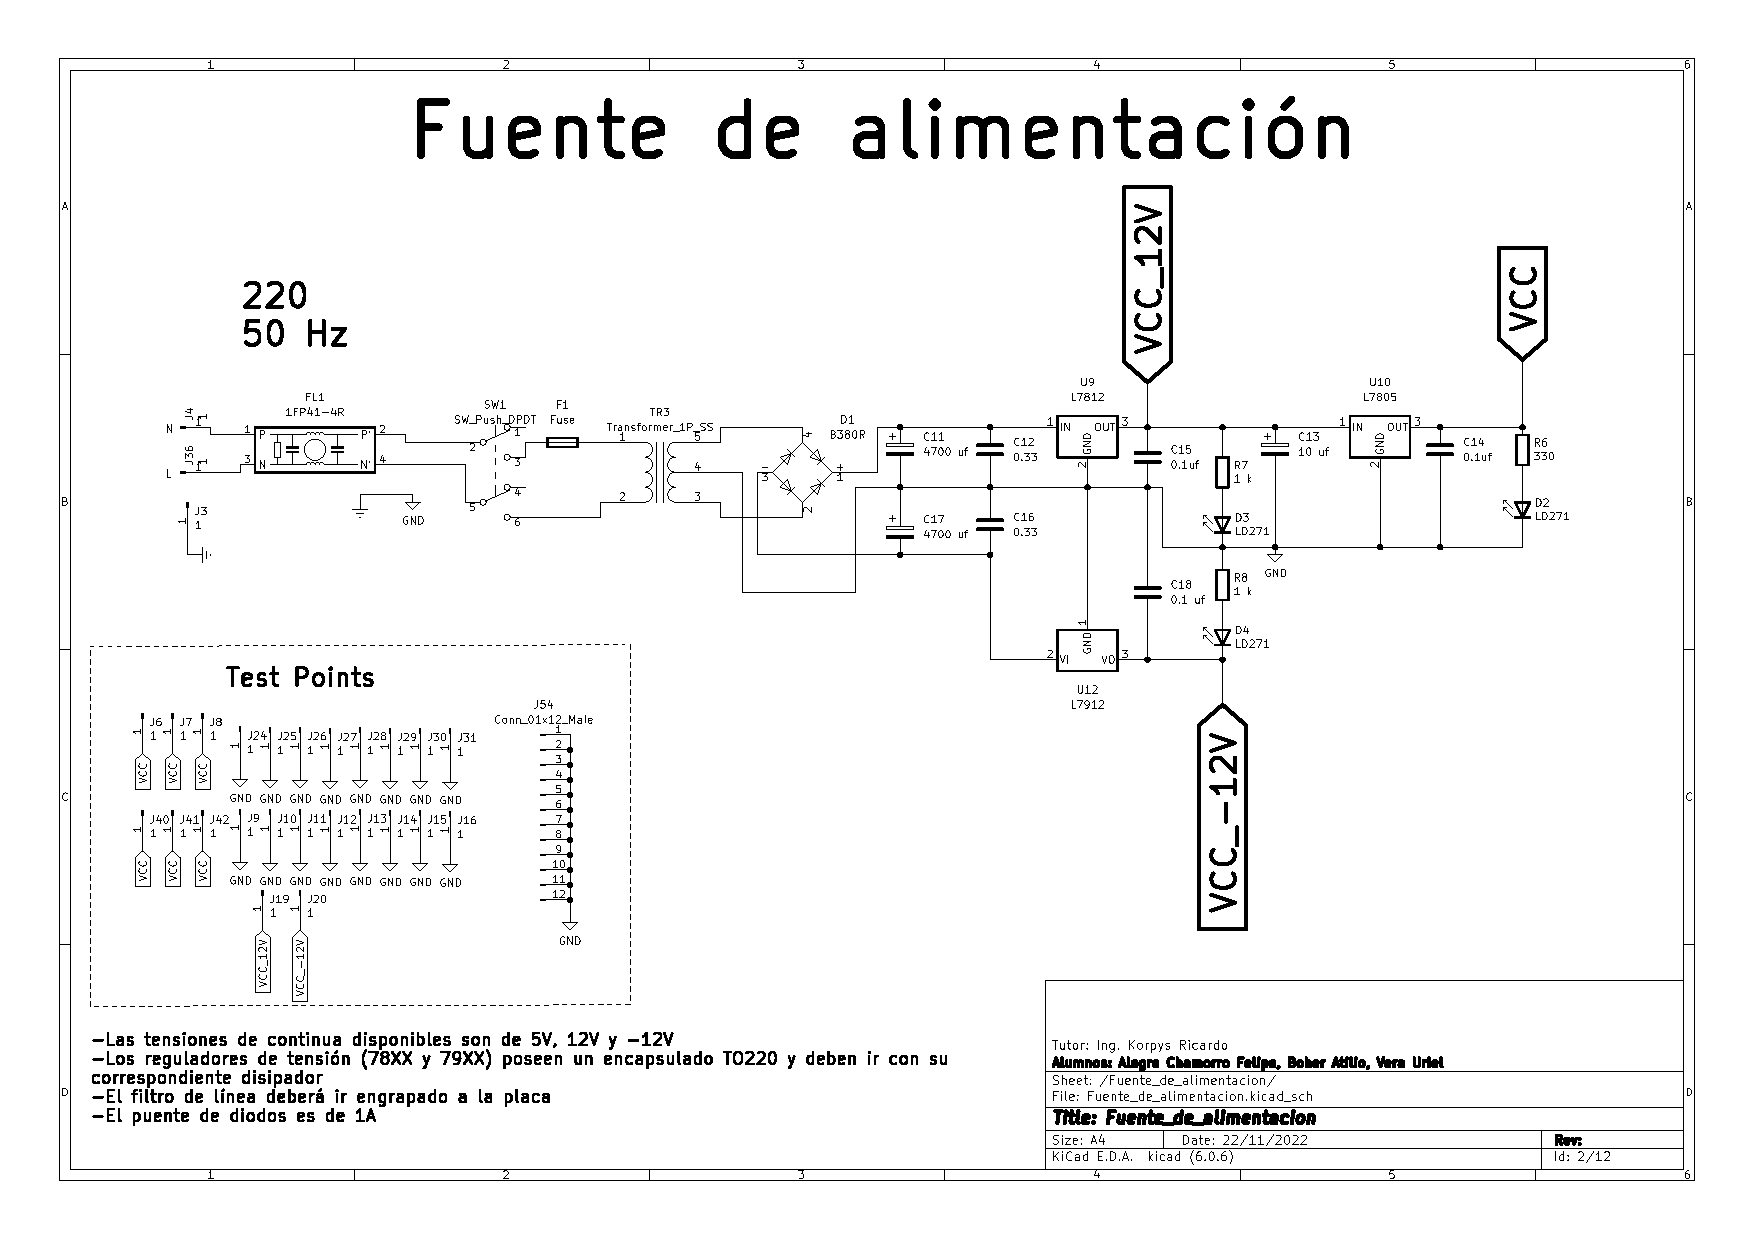
\includegraphics[width=1.2\textwidth, angle=90]{./imagenes/EsquematicosSF/Esquematico (2).pdf}
  \caption{Esquema de fuente de alimentación de sistema final}
  \label{F:EsqSF2}
\end{figure}

\clearpage
\subsection{Mapa de memoria}
El planteo establecido para el mapa de memoria consta de dos modos de operación, un modo de inicio y un modo de ejecución o RUN. El sistema fue pensado de esta manera para tener disponible más memoria RAM en ejecución. 

El modo inicio consiste en la memoria EEPROM 28C256 en la primera mitad del mapa de memoria (0000h a 7FFFh) y en la segunda mitad una memoria RAM en dos tramos de 8000h a F7FFh y luego continúa en FC00h hasta FFF8h, se interrumpe de esta manera la RAM para simplificar el circuito decodificador el cual se presenta más adelante (Sección \ref{C:Decodificador}). La sección del mapa de memoria de F800h hasta FBFFh es destinada a la comunicación SPI. Y finalmente, en la zona superior del mapa de memoria (FFF8h a FFFFh), la memoria RAM DALLAS 1744 posee un apartado para un reloj de tiempo real. 

El modo de ejecución es un modo en el cual se cambia la primera mitad del mapa de memoria (0000h a 7FFFh). El proceso consiste en cambiar la memoria EEPROM del modo de inicio por una memoria RAM. Este proceso debe ser ejecutado por software y para ello en el modo de inicio se debe copiar el contenido de la memoria EEPROM en la RAM1, luego el sistema seguirá funcionando con la memoria de programa en la RAM1 y en la primera mitad del mapa de memoria se tendrá disponible la memoria RAM2. 

\begin{figure}[ht]
  \centering
  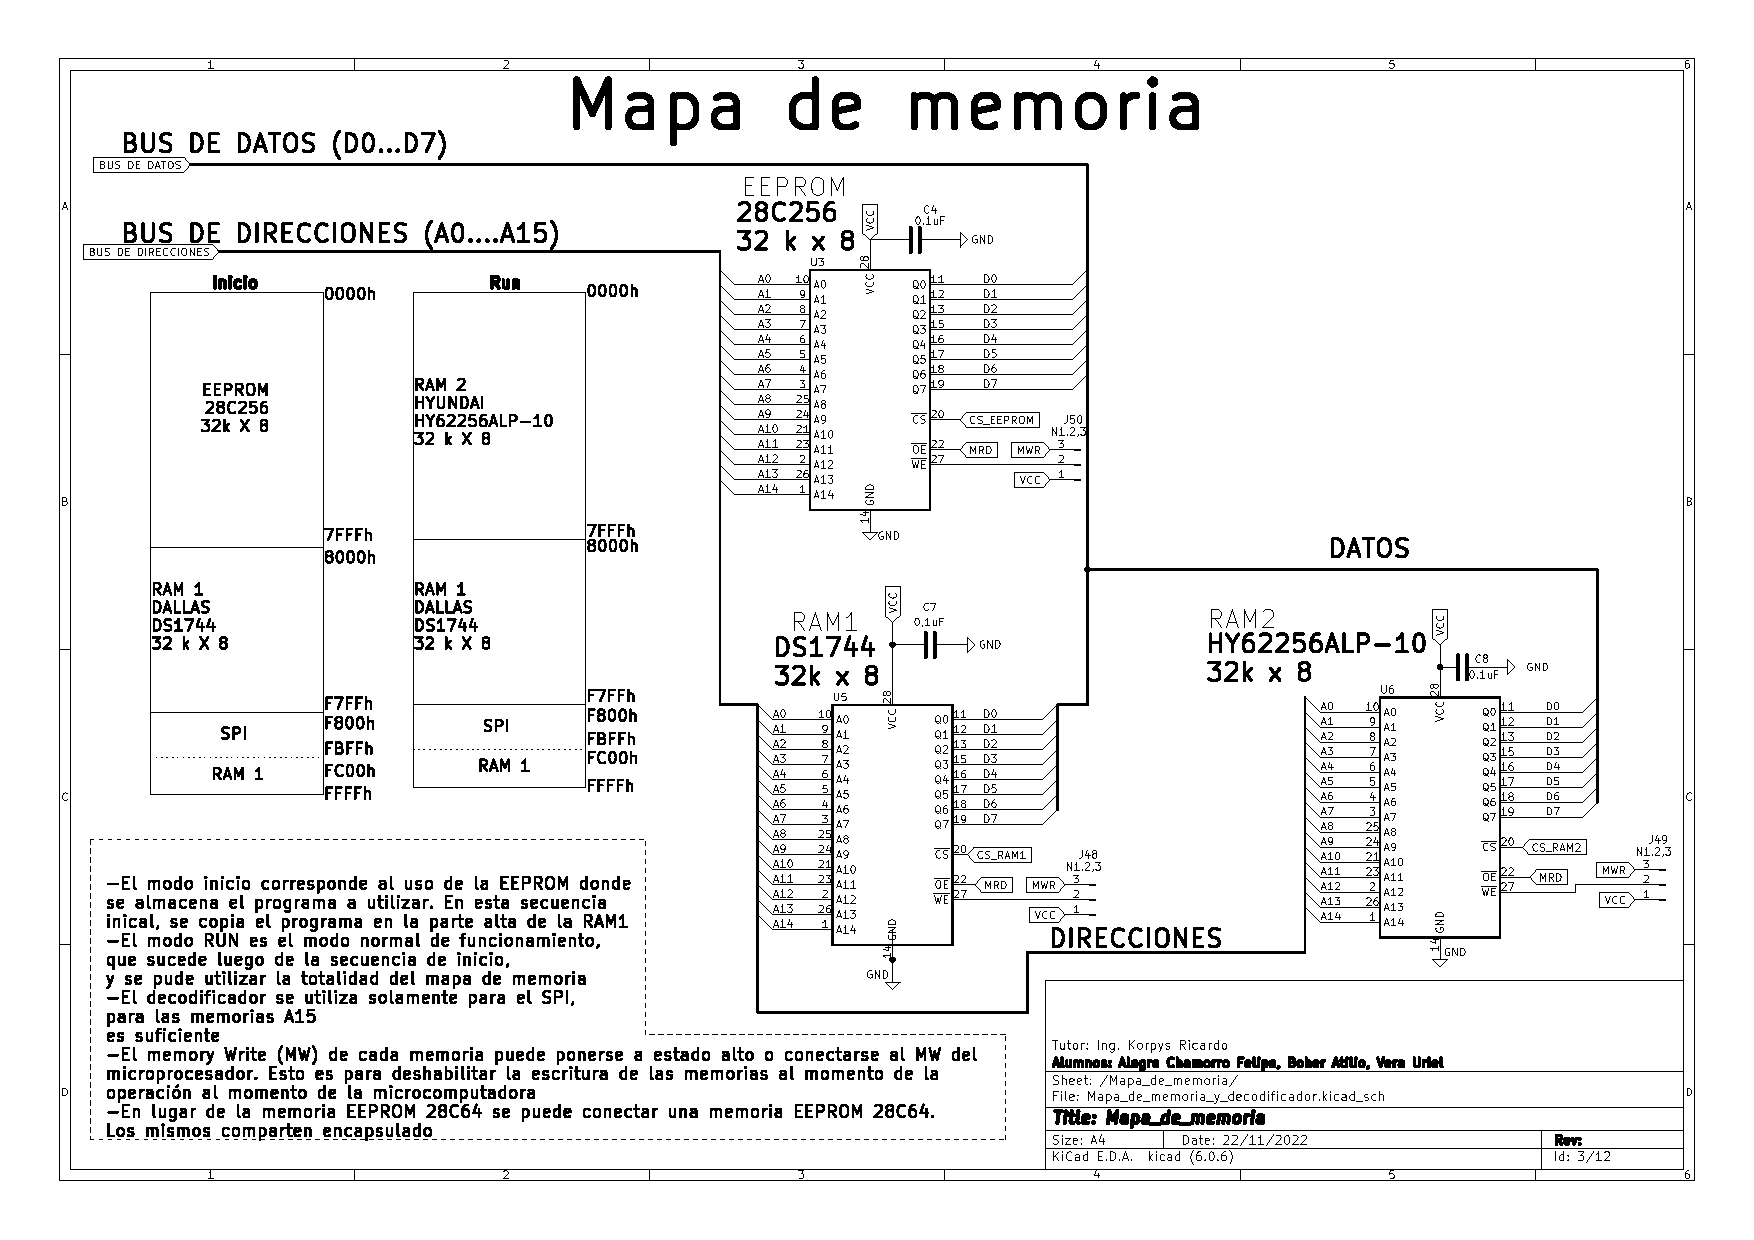
\includegraphics[width=1.2\textwidth, angle=90]{./imagenes/EsquematicosSF/Esquematico (3).pdf}
  \caption{Esquema de Mapa de memoria de sistema final}
  \label{F:EsqSF3}
\end{figure}

\clearpage
\subsection{Memorias seriales}
El trabajo con memorias seriales fue planteado para diferentes tecnologías de memorias, específicamente del tipo EEPROM, FRAM y SDcard. Para la comunicación I2C se prevé el uso de un sistema de comunicación por software utilizando la interfaz de entrada salida presentada en la sección \ref{C:I/O} e interactuando con el acondicionamiento presentado en \ref{C:BUSI2C}, mientras que para la comunicación SPI, se diseñó un sistema por hardware presentado en la sección \ref{C:esqSPI}. En el esquema de la figura \ref{F:EsqSF4} se observan las etiquetas de interconexión con el resto del circuito.
\begin{figure}[ht]
  \centering
  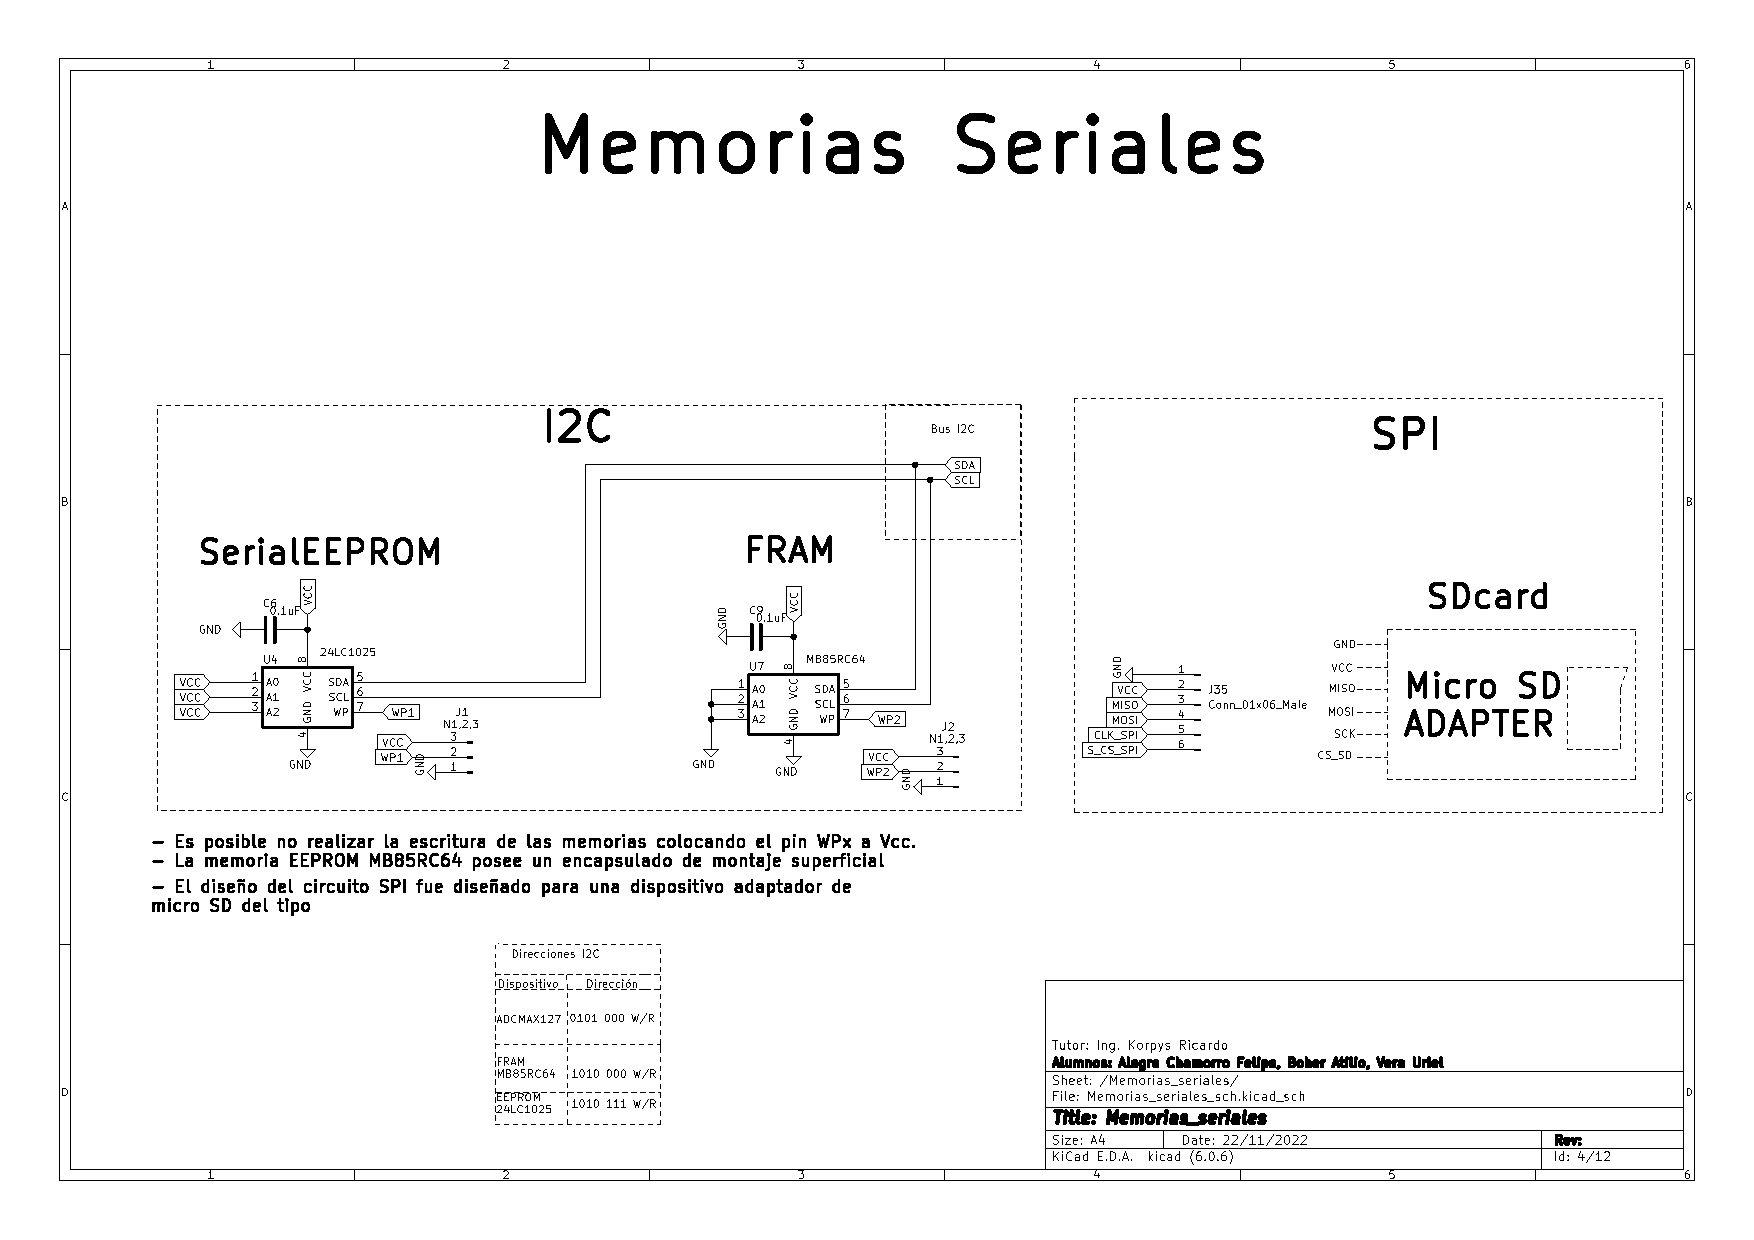
\includegraphics[width=1.2\textwidth, angle=90]{./imagenes/EsquematicosSF/Esquematico (4).pdf}
  \caption{Esquema de memorias seriales de sistema final}
  \label{F:EsqSF4}
\end{figure}

\clearpage
\subsection{Conversor analógico digital}

El sistema de conversión analógico-digital se basa en el MAX127 \cite{datasheet_max127}. Este conversor de 12 bits es configurable, lo que permite seleccionar el rango de tensiones a medir por cada canal y se realiza mediante comunicación I2C. Los rangos de medición pueden ser:
\begin{itemize}
    \item 0~V a 5~V
    \item -5~V a 5~V
    \item 0~V a 10~V
    \item -10~V a 10~V
\end{itemize}

Para el acondicionamiento de señal se utilizan amplificadores operacionales OPA4277~\cite{datasheet_OPA4277}. Los amplificadores operacionales se configuraron como conversores de corriente a tensión, de 4-20~mA a 0-10~V. Se concibió el diseño de esta manera, ya que en caso de que se requiera medir tensiones, el circuito puede ser modificado para que los amplificadores operacionales funcionen como seguidores de tensión. Basta con modificar el rango de medición por software para que la lectura refleje correctamente el valor a la entrada. 

\begin{figure}[ht]
  \centering
  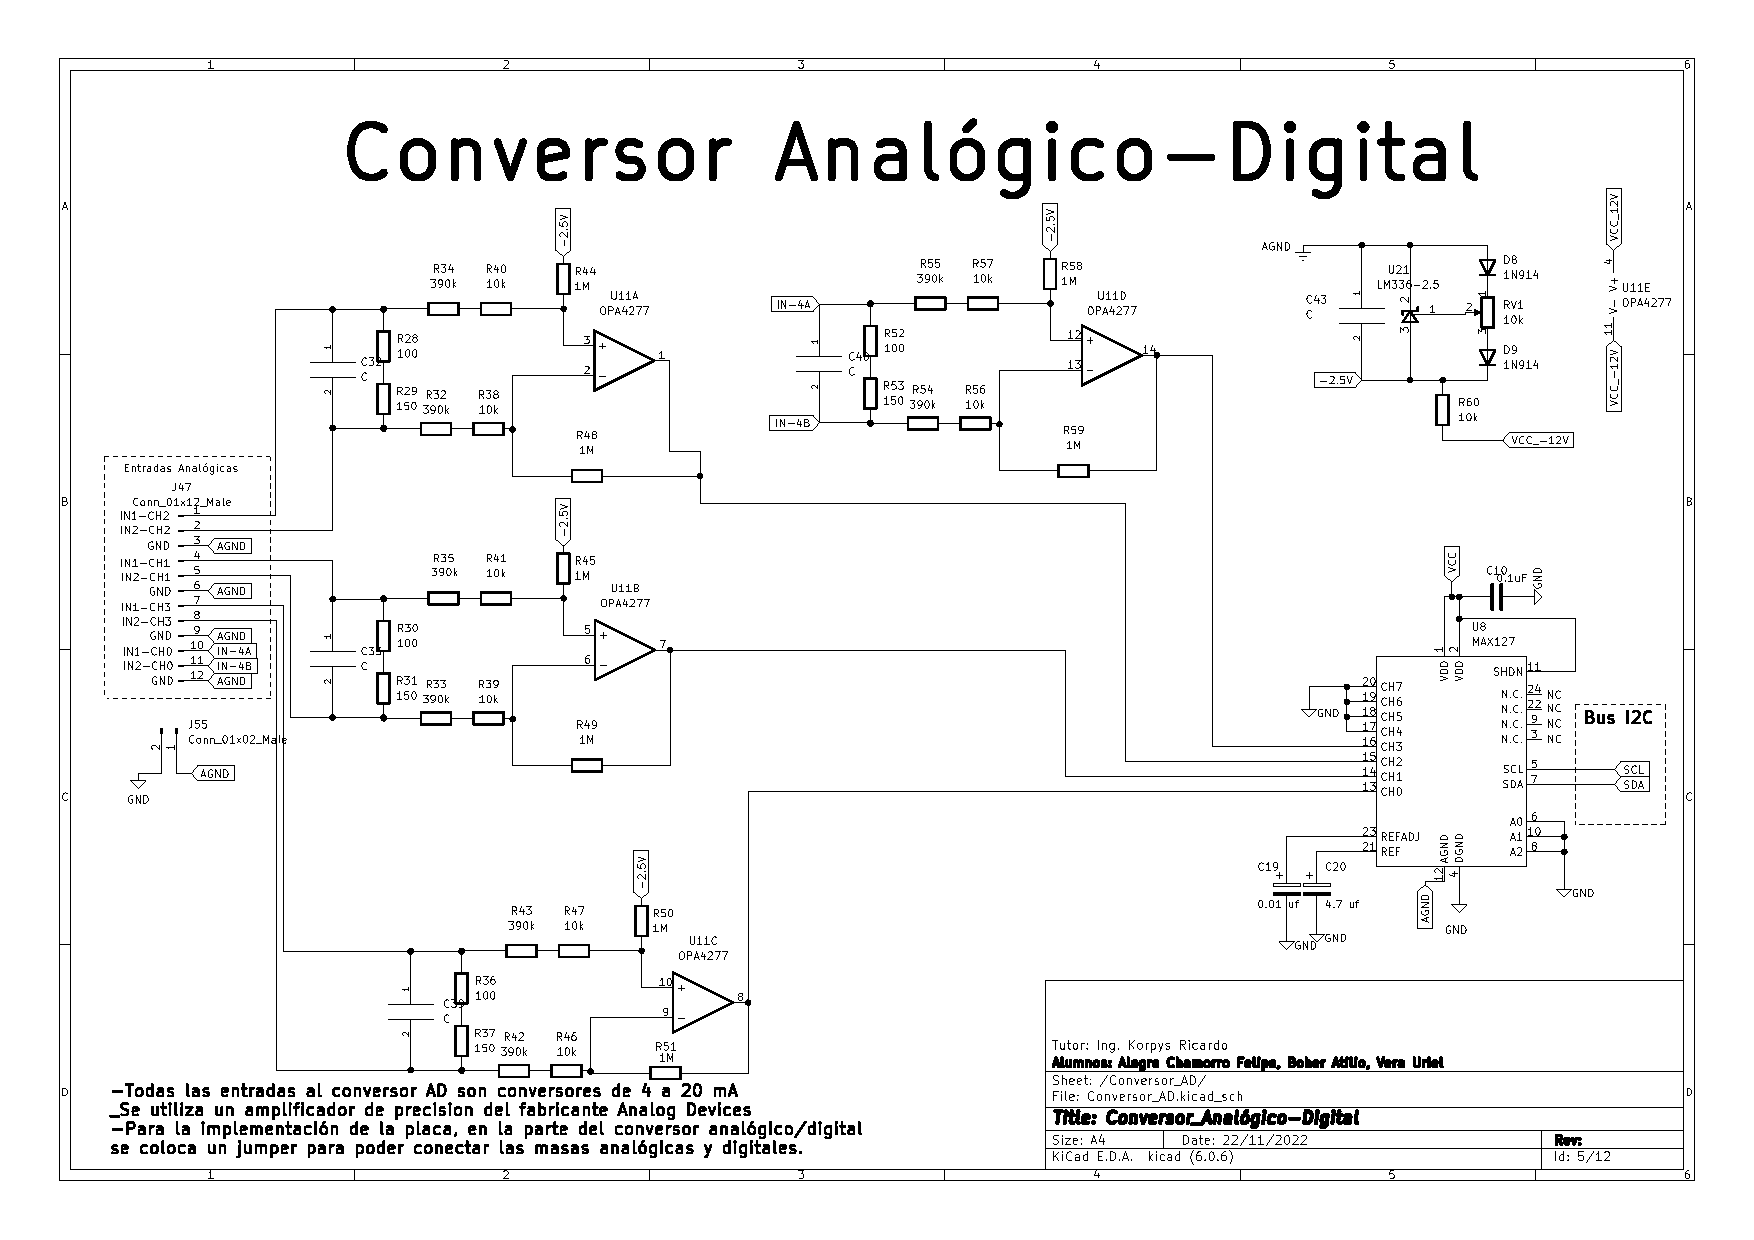
\includegraphics[width=1.2\textwidth, angle=90]{./imagenes/EsquematicosSF/Esquematico (5).pdf}
  \caption{Esquema de conversor analógico digital de sistema final}
  \label{F:EsqSF5}
\end{figure}

\clearpage
\subsection{Microprocesador}
En el esquema del microprocesador se observa su interacción con el resto del circuito. Es interesante destacar el latch 74HC573~\cite{datasheet_74HC573} el cual se encarga de transmitir los bits más significativos del bus de direcciones (A8-A15), esta configuración de microprocesador/latch para el direccionamiento es propia de la arquitectura propuesta por el CDP1802. Sin embargo, se utiliza un circuito integrado distinto al del sistema medio ya que su distribución de pines permite simplificar el diseño de la placa PCB. En el esquema también se puede observar una interfaz de usuario compuesta por pulsadores para señal de entrada y LEDs para señal de salida. 
El circuito oscilador que se presenta en el esquema está construido a partir de un cristal de 4~MHz. Es importante destacar que en la hoja de datos del microprocesador la frecuencia máxima para las condiciones de trabajo que establecemos es de 3,2~MHz, sin embargo, en la práctica es utilizado a mayor frecuencia y existen muchos casos prácticos que corroboran el funcionamiento con overclocking, como en la computadora Membership Card mencionada anteriormente \cite{membership-card}. 

\begin{figure}[ht]
  \centering
  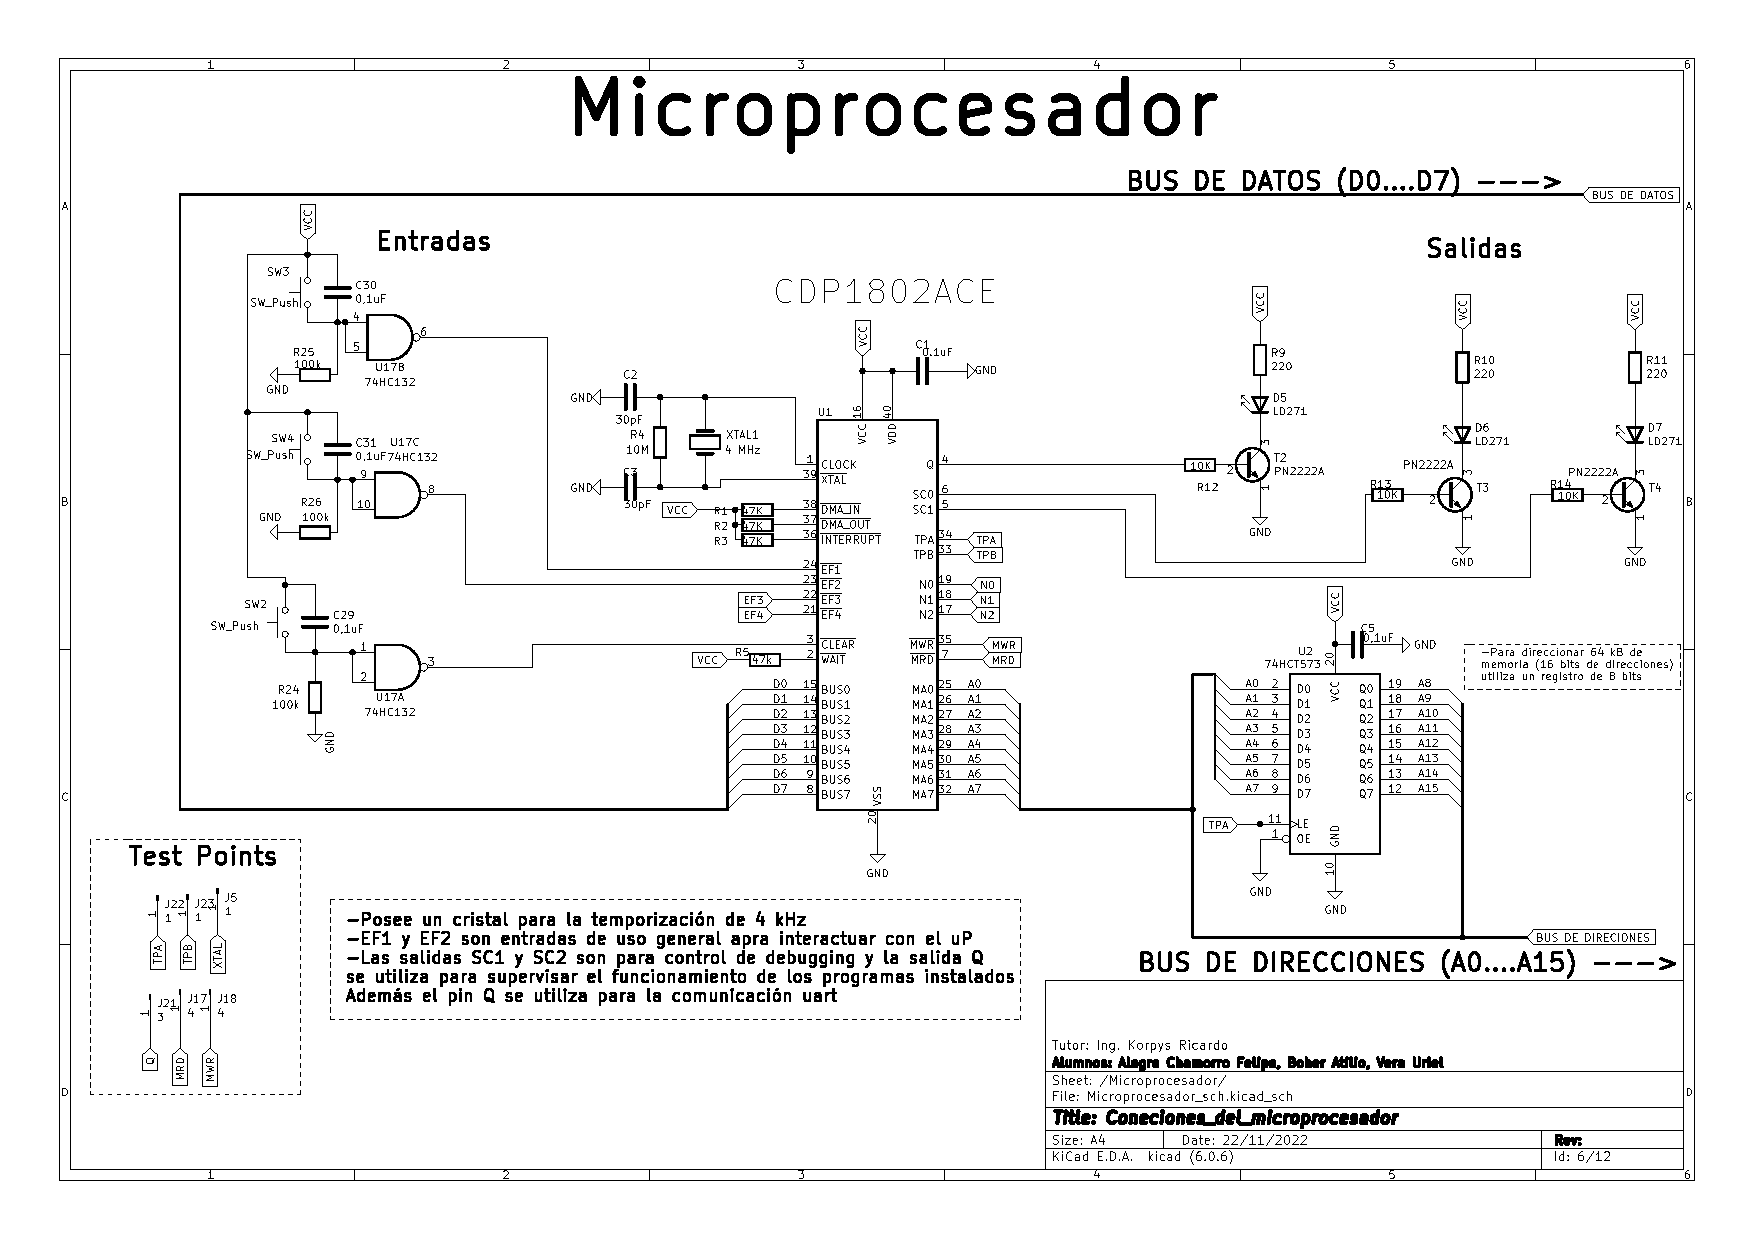
\includegraphics[width=1.2\textwidth, angle=90]{./imagenes/EsquematicosSF/Esquematico (6).pdf}
  \caption{Esquema de conexión de microprocesador de sistema final}
  \label{F:EsqSF6}
\end{figure}

\clearpage
\subsection{Decodificador}
\label{C:Decodificador}

El circuito decodificador se encarga de activar la selección de los dispositivos según lo presente en el bus de direcciones. Para ello se utiliza un circuito lógico con compuertas y un decodificador de 3 líneas a 8 líneas 74HC138 \cite{datasheet_74HC138}.

\begin{figure}[ht]
  \centering
  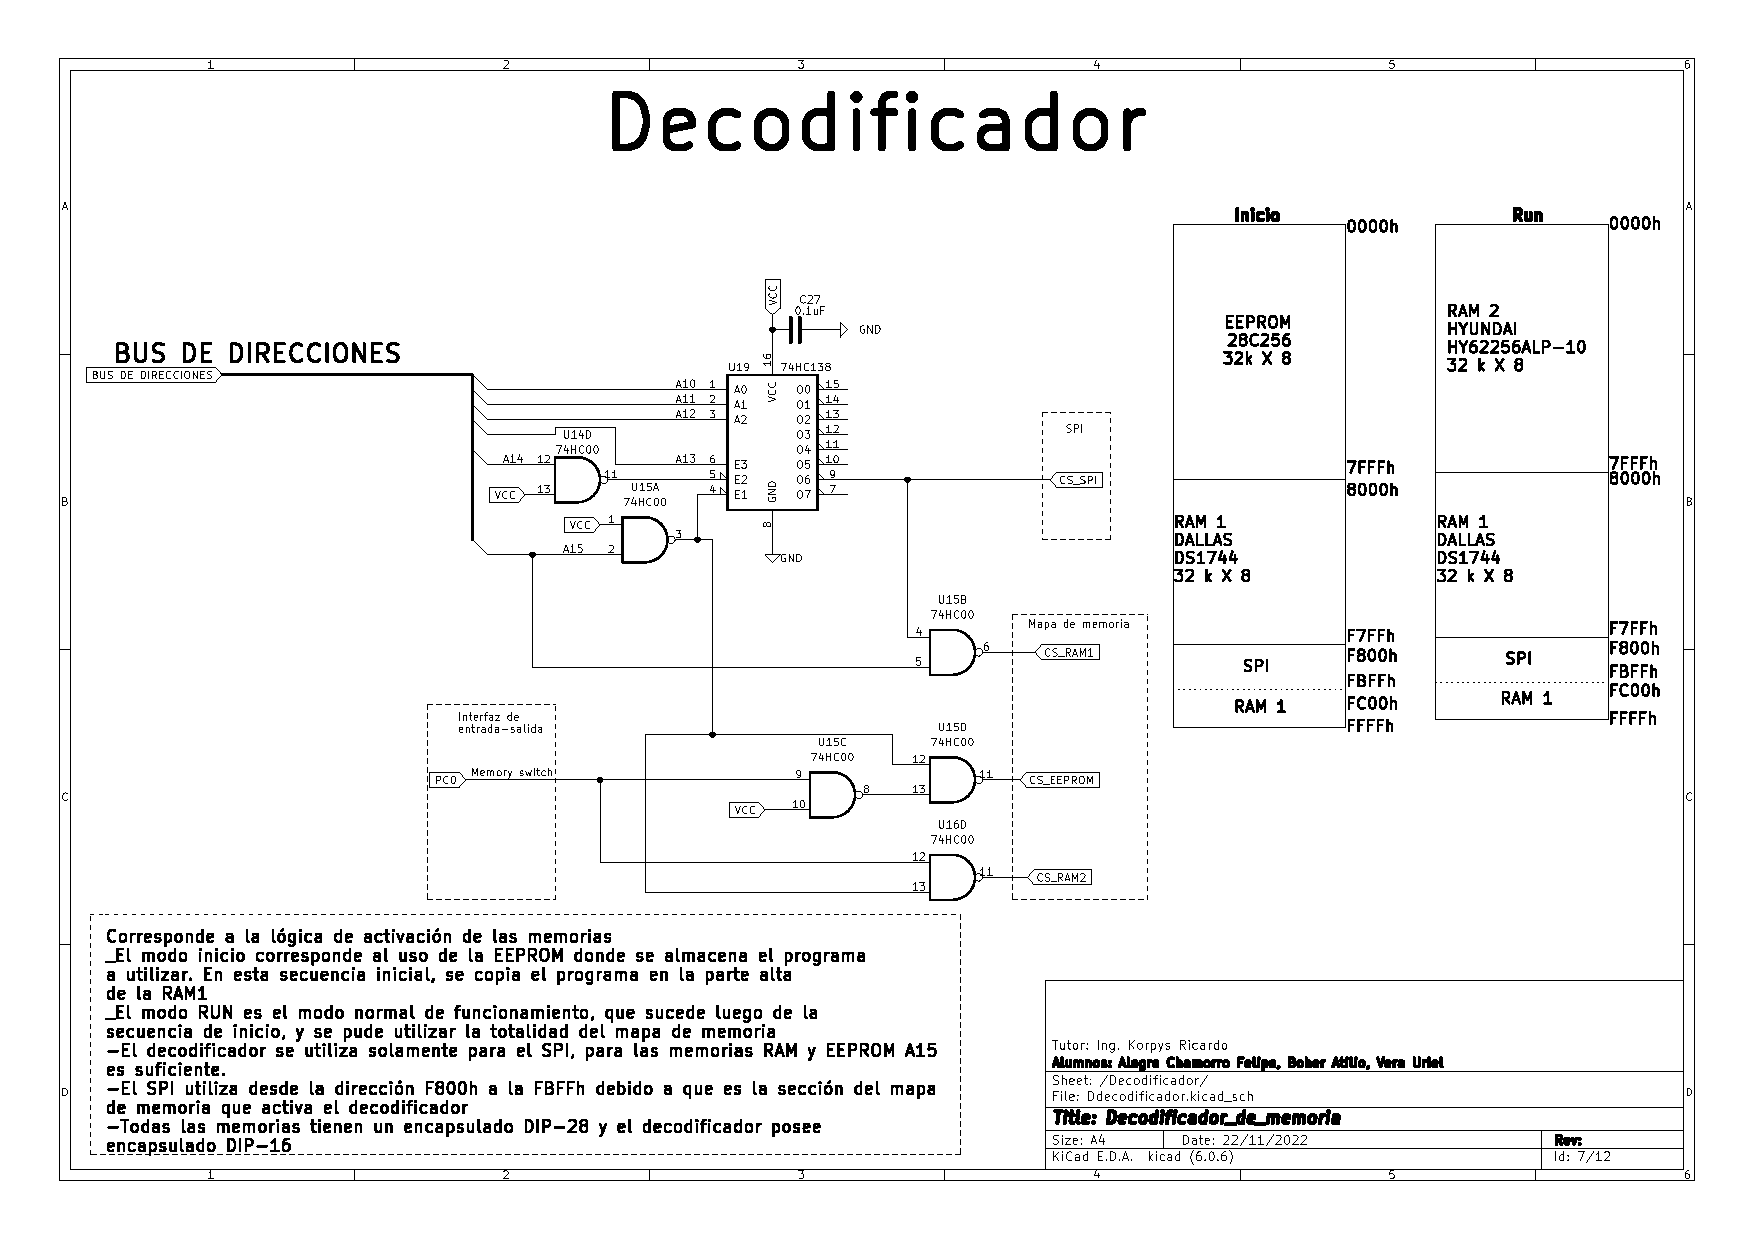
\includegraphics[width=1.2\textwidth, angle=90]{./imagenes/EsquematicosSF/Esquematico (7).pdf}
  \caption{Esquema de decodificador de memoria de sistema final}
  \label{F:EsqSF7}
\end{figure}

\clearpage
\subsection{Comunicación UART}

La comunicación UART se basa principalmente en el software que la controla y se utiliza el pin Q del microprocesador para la transmisión de datos. Para lograr establecer comunicación con una terminal en una computadora personal se requiere la conexión por medio de USB, por lo que se conecta una interfaz FT232RL~\cite{datasheet_FT232RL} que realiza la interpretación y retransmisión de los protocolos. 

\begin{figure}[ht]
  \centering
  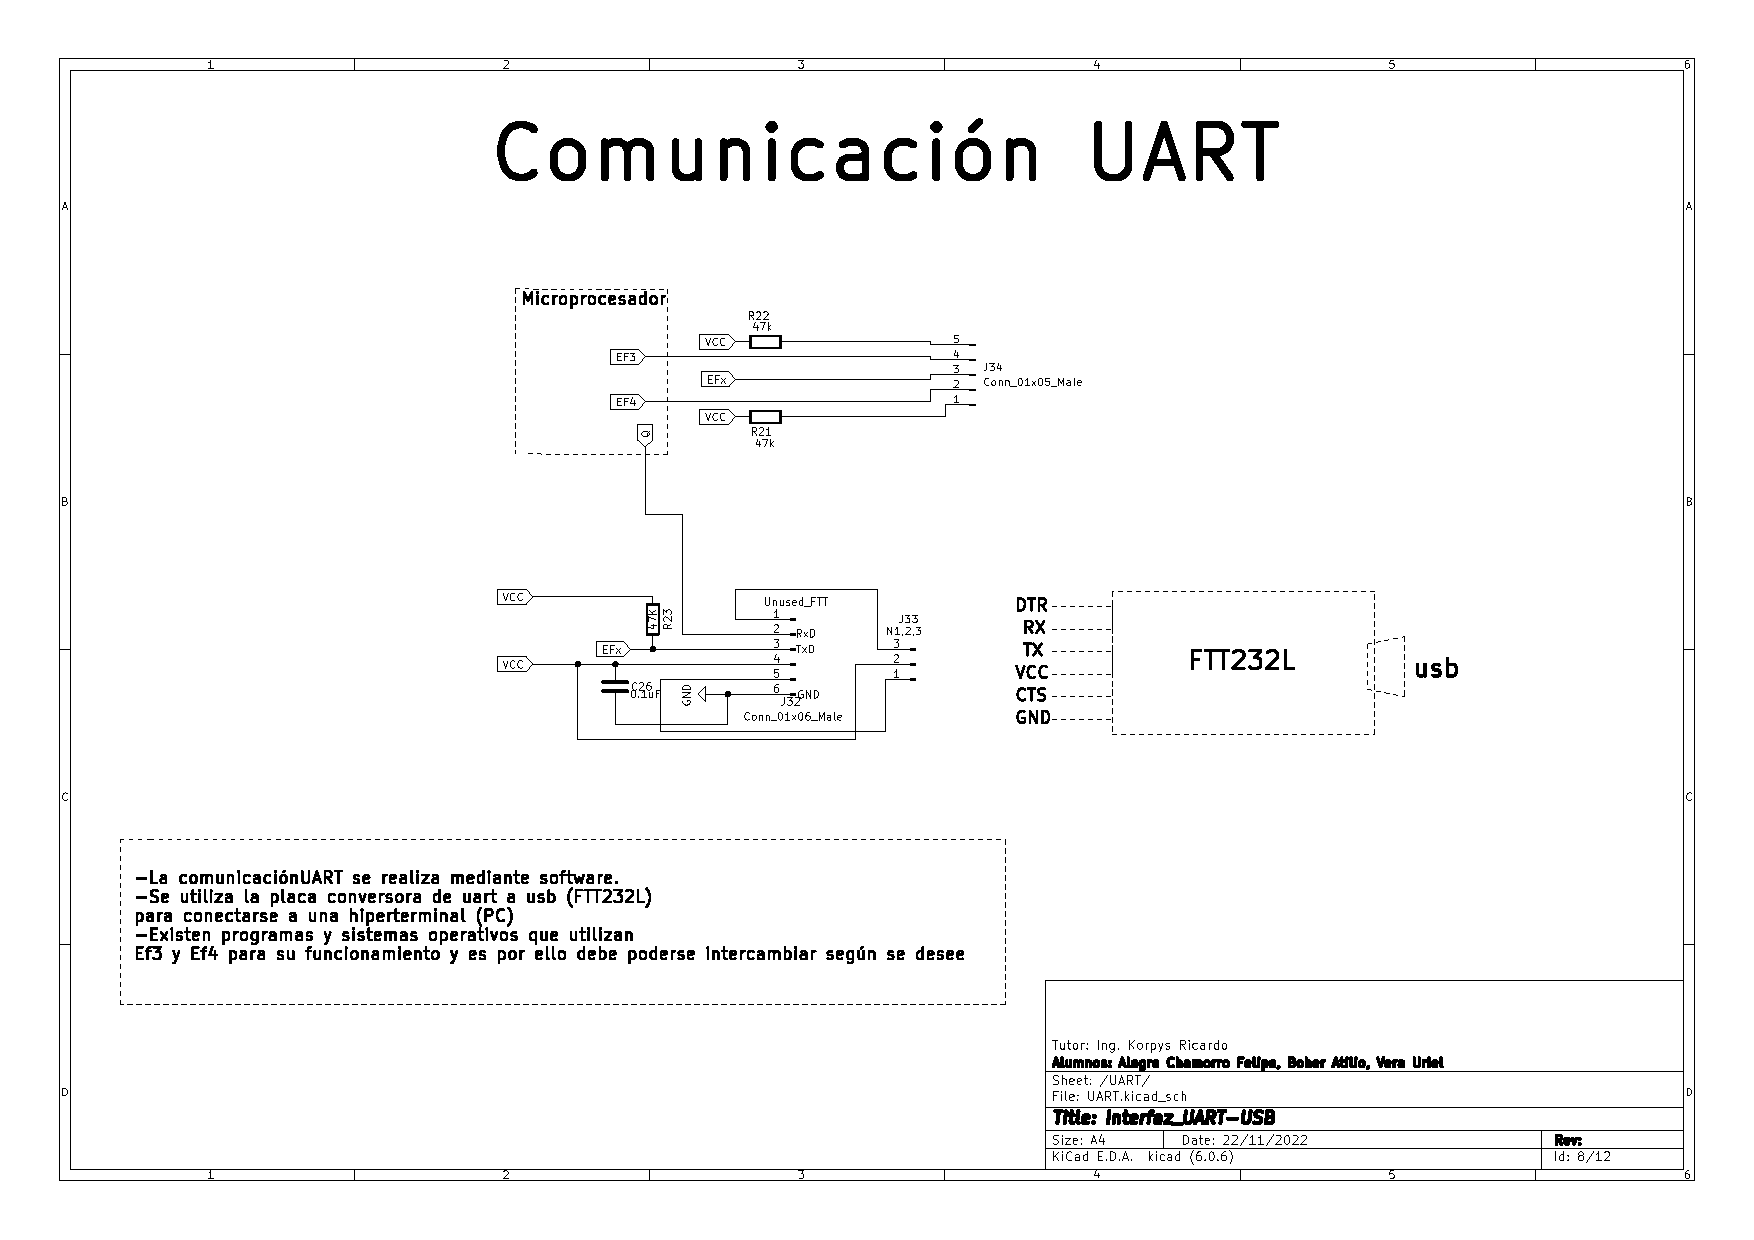
\includegraphics[width=1.2\textwidth, angle=90]{./imagenes/EsquematicosSF/Esquematico (8).pdf}
  \caption{Esquema de comunicación UART de sistema final}
  \label{F:EsqSF8}
\end{figure}

\clearpage
\subsection{Comunicación SPI}
\label{C:esqSPI}

En el esquemático de la figura~\ref{F:EsqSF9} se observa un circuito diseñado para realizar una comunicación basada en el protocolo SPI. Fue planteado con el objetivo de simplificar el procesamiento de datos en el microprocesador, realizándose un gran número de iteraciones en el circuito de manera transparente para el procesador. 

En principio se debe considerar que el sistema planteado cuenta con una señal de reloj proveniente de un cristal oscilador compatible con CMOS. Este cristal, al igual que el conectado al microprocesador, es de 4~MHz. Considerando que las instrucciones en el procesador duran 8 ciclos de reloj, se tendrá una velocidad de procesamiento mayor en el hardware diseñado. Esto se representa más adelante en los diagramas temporales. 

Básicamente el sistema presentado consiste en hacer trabajar 2 registros de desplazamiento (shift-register), uno para enviar datos y el otro para recibirlos. 

Para el envío de datos se utiliza un registro de desplazamiento de entrada paralela y salida serie, el MC14014 \cite{datasheet_MC14014B} (también se encuentra como CD4014). Este dispositivo cuenta con un registro interno el cual guarda el dato disponible en el bus al recibir una señal en estado alto en el pin PL. La lectura de los puertos de entrada se realiza con la señal de clock, por lo que para el guardado de los datos en el bus se debe detectar un flanco ascendente en el pin CP. Una vez guardado el dato en el registro, se encuentra listo para transmitirlo, este proceso se acciona con una señal de estado bajo en el pin PL y se transmite de manera serial con las transiciones positivas de la señal de reloj. 

Para la recepción de datos se utiliza un registro de desplazamiento de entrada serial y salida paralelo, el 74HC595 \cite{datasheet_74HC595}. Este dispositivo cuenta con una entrada serial, por la cual toma el dato a almacenar, realizando una lectura en dicha entrada por cada flanco de reloj detectado. El dato presente en el registro de desplazamiento varía por cada ciclo de reloj, por lo que al transcurrir 8 ciclos se encuentra completo el registro, para guardar este dato y que no se vea alterado por el transcurso de los posteriores ciclos, se utiliza el pin RCLK que permite guardar el dato en un registro paralelo. Para que este dato sea presentado en la salida paralelo, se pone en estado bajo el pin de output enable $\overline{\text{OE}}$.

La señal de clock utilizada para los integrados mencionados anteriormente se genera a partir del circuito establecido entre el cristal oscilador, el flip flop D 74HC74, el contador 74HC161 y el flip flop JK 74HC73 \cite{datasheet_74HC161, datasheet_74HC73, datasheet_74HC74}. La topología presentada en el esquema detecta el inicio del ciclo al recibir la señal proveniente de PC7, poniendo en estado alto el pin 4 del 74HC74, la señal generada por Q inicializa el contador. En el contador se toma la señal Q0 como señal de reloj, la cual tendrá una frecuencia de 2~MHz y luego cuando el contador se desborda la salida TC se pone en alto, esta señal es resguardada por el flip flop 74HC73 y utilizada como señal de reinicio del flip flop 74HC74. De esta manera se genera una señal oscilante de 2~MHz a la salida pero que solo tiene 8 pulsos, lo necesario para realizar el envío de un byte. 

\begin{figure}[ht]
  \centering
  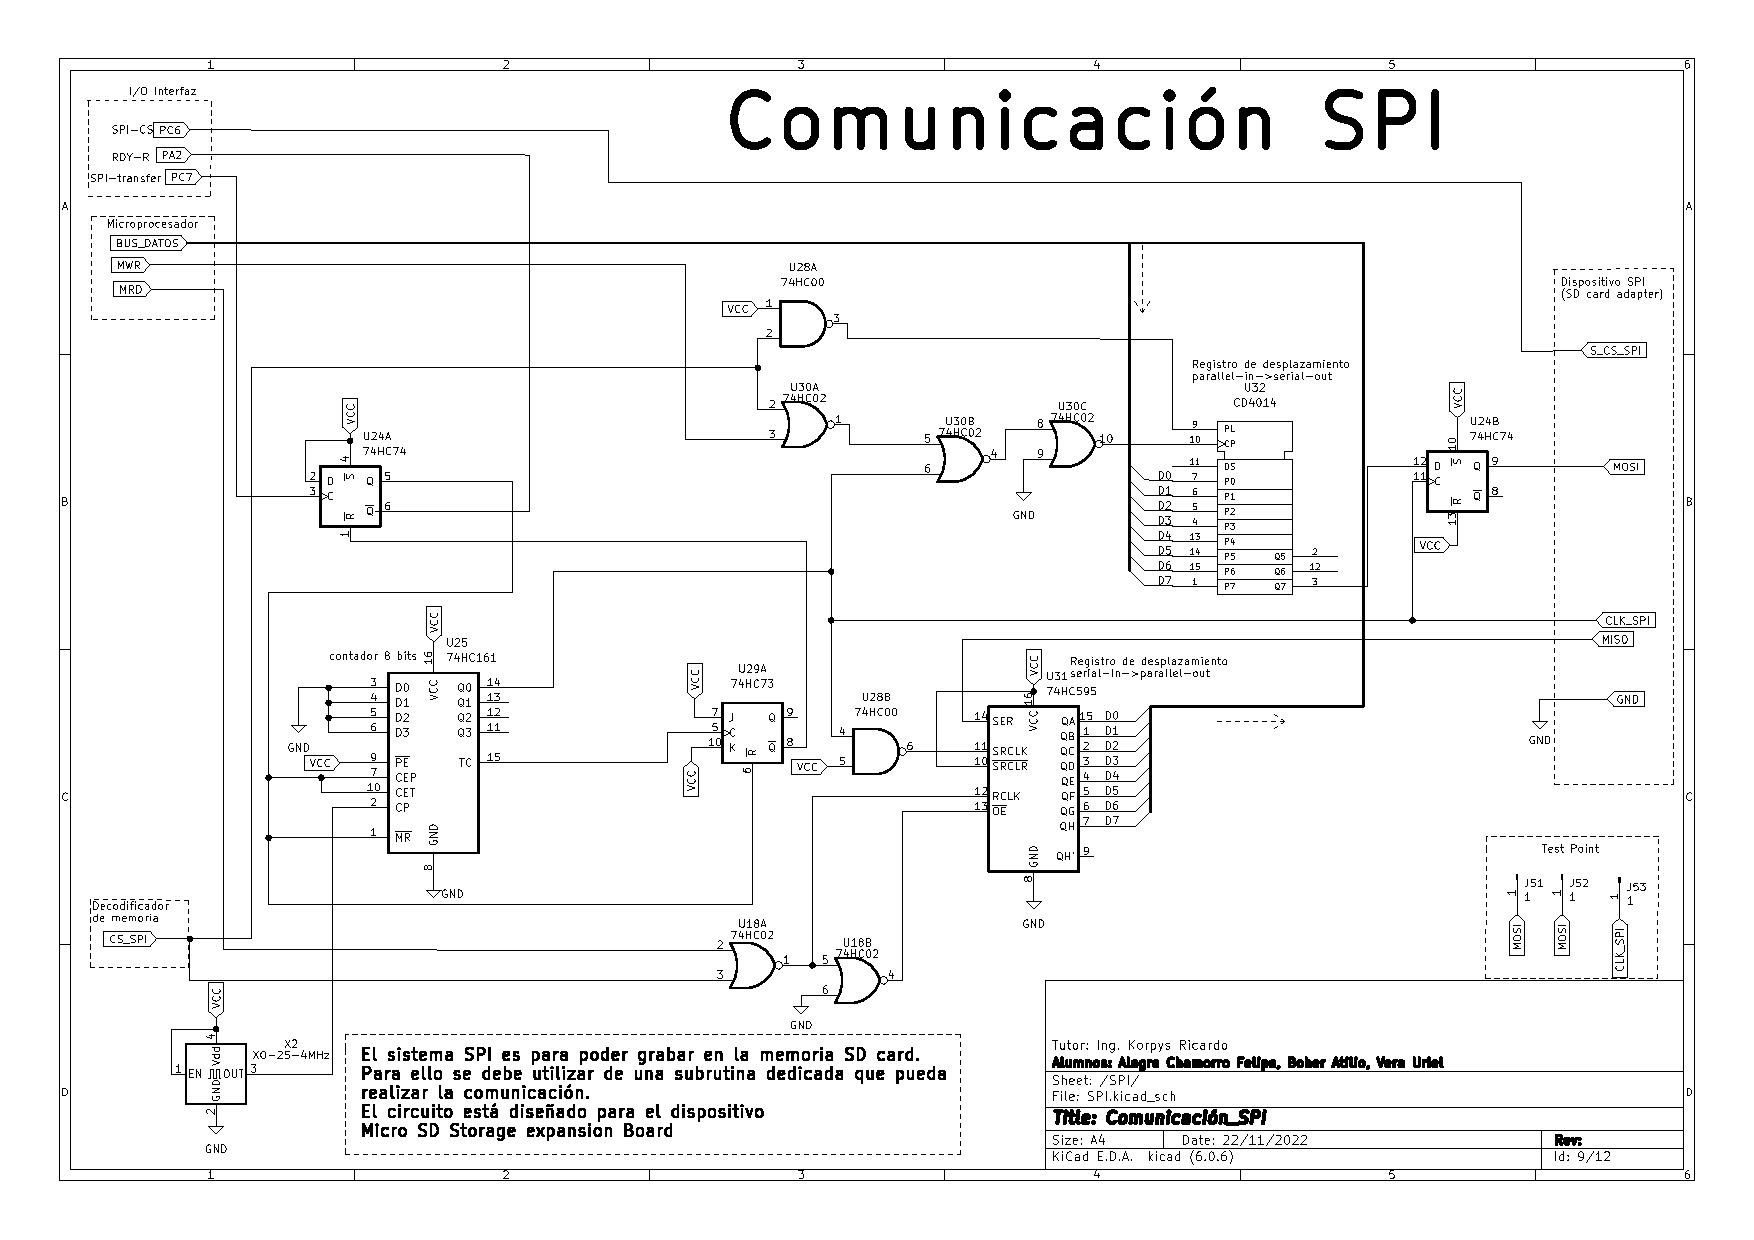
\includegraphics[width=1.2\textwidth, angle=90]{./imagenes/EsquematicosSF/Esquematico (9).pdf}
  \caption{Esquema de comunicación SPI de sistema final}
  \label{F:EsqSF9}
\end{figure}

Para el control del sistema se desarrolló un algoritmo simple el cual se presenta en el listado \ref{L:instrucciones_V3}. El funcionamiento general de este sistema se puede desglosar en tres partes. El proceso en el cual se guarda el dato a transmitir, presentado en la figura~\ref{F:DT1_SPI}; la transmisión, presentada en la figura~\ref{F:DT2_SPI}, y la lectura del dato recibido, presentada en la figura~\ref{F:DT3_SPI}. El código assembler presentado en los gráficos se corresponde con el algoritmo presentado en el listado \ref{L:instrucciones_V3}.

\begin{figure}[H]
  \centering
  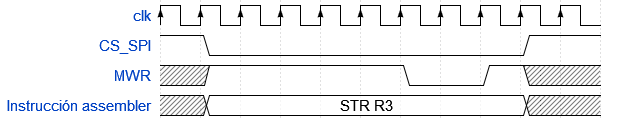
\includegraphics[width=0.55\textwidth]{./imagenes/EscrituraSPI.png}
  \caption{Proceso de guardado de dato a transmitir}
  \label{F:DT1_SPI}
\end{figure}

\begin{figure}[H]
  \centering
  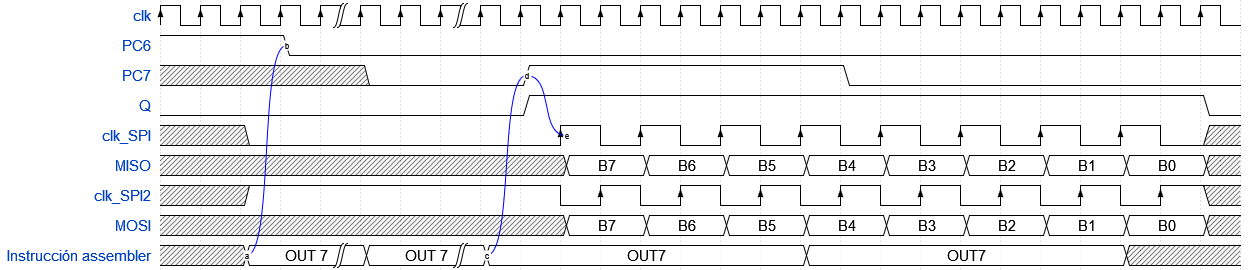
\includegraphics[width=1\textwidth]{./imagenes/TransmisionSPI.png}
  \caption{Proceso de transmisión SPI}
  \label{F:DT2_SPI}
\end{figure}

\begin{figure}[H]
  \centering
  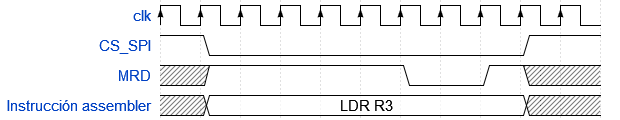
\includegraphics[width=0.55\textwidth]{./imagenes/LecturaSPI.png}
  \caption{Proceso de lectura}
  \label{F:DT3_SPI}
\end{figure}

\clearpage
\footnotesize
\lstinputlisting[language=CDP1802, caption={\centering Rutina propuesta para la transmisión utilizando el circuito de comunicación SPI}, label = {L:instrucciones_V3}]{codigo/instrucciones_V3.asm}
\normalsize

\clearpage
\subsection{Alimentación de compuertas}
La alimentación de compuertas es un esquemático en el cual se representan los puntos de alimentación de los circuitos integrados y los elementos no usados de los dispositivos electrónicos. Principalmente sirve para tener una vista más limpia en los demás esquemas.

\begin{figure}[ht]
  \centering
  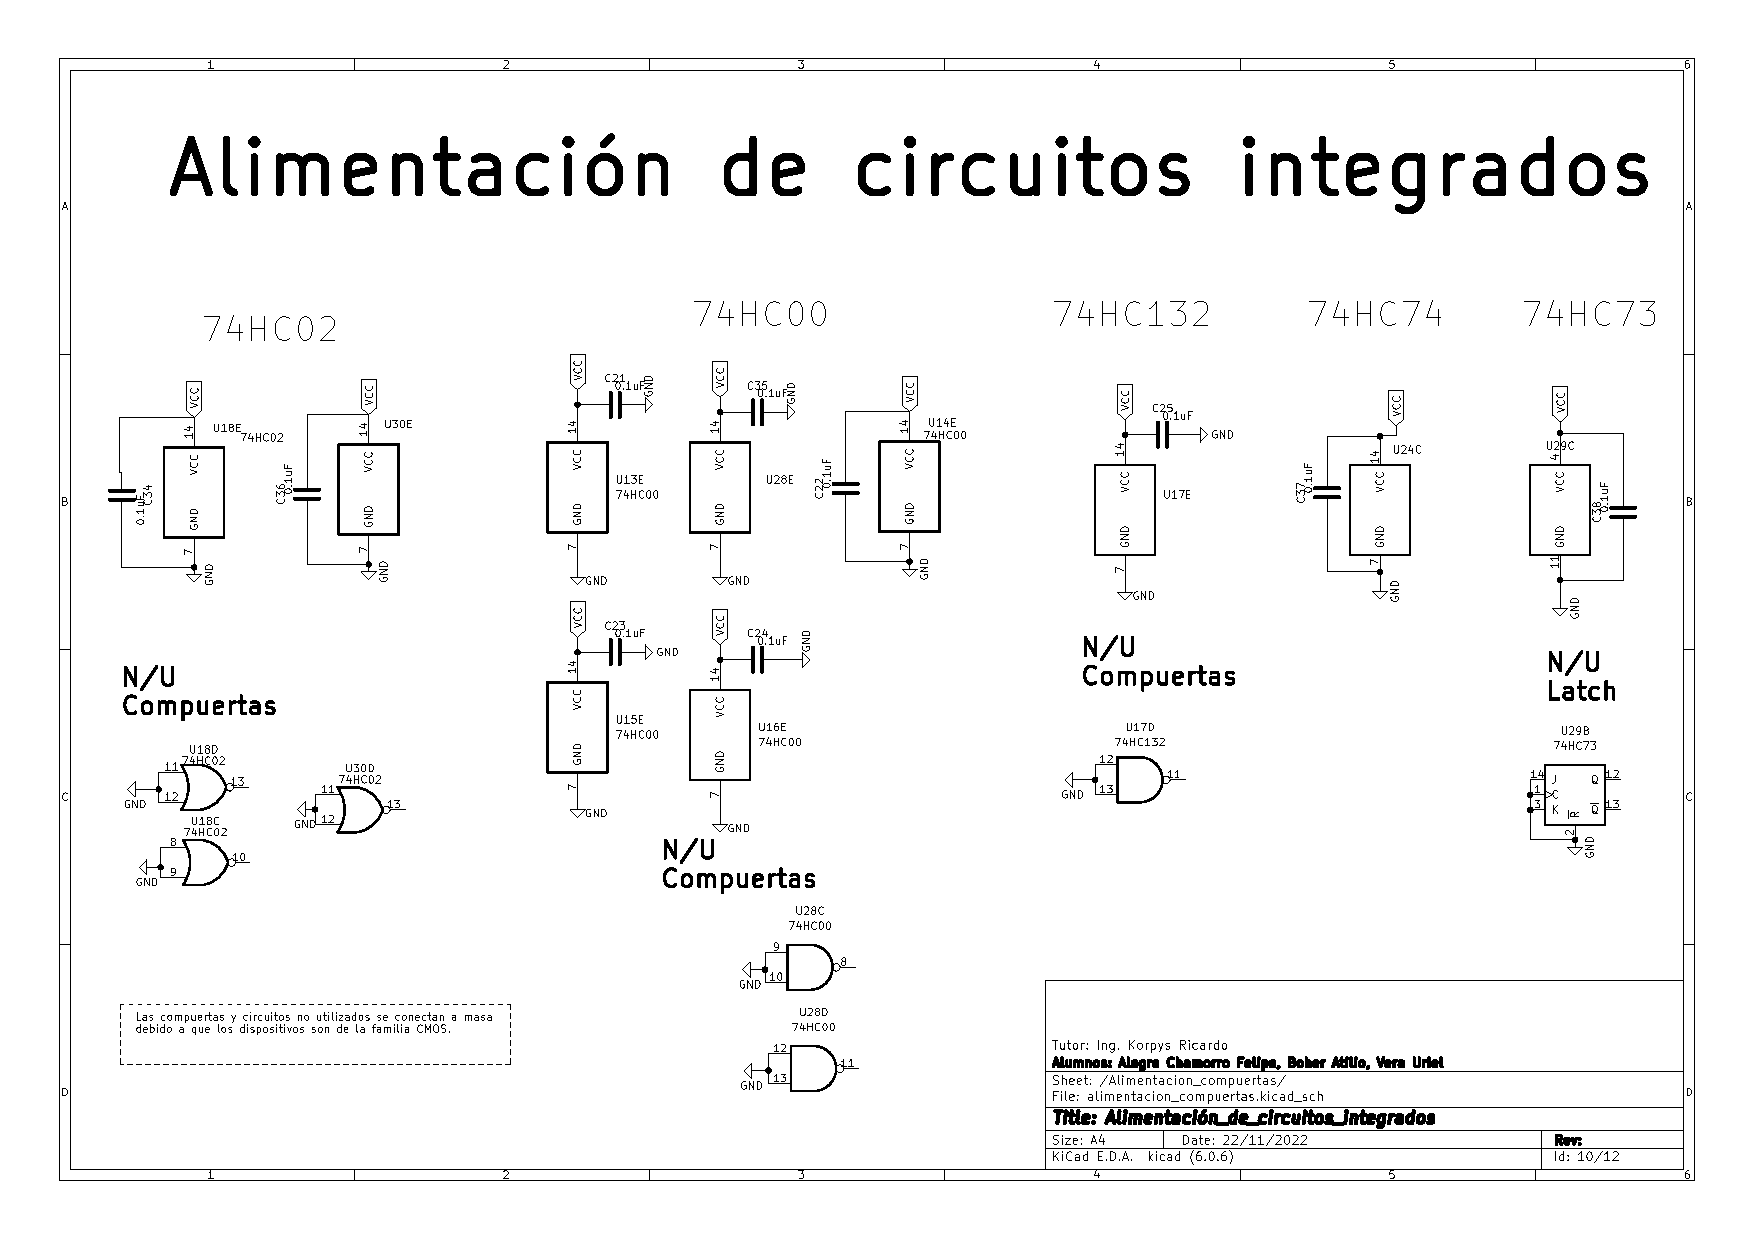
\includegraphics[width=1.2\textwidth, angle=90]{./imagenes/EsquematicosSF/Esquematico (10).pdf}
  \caption{Esquema de alimentación de compuertas de sistema final}
  \label{F:EsqSF10}
\end{figure}

\clearpage
\subsection{Interfaz I/O}
\label{C:I/O}

El microprocesador CDP1802 posee una arquitectura poco común, la cual cuenta con un mapa de memoria separado para los dispositivos de entrada y salida. Esto le da la capacidad al microprocesador de poder acceder a la memoria y a los dispositivos de entrada y salida al mismo tiempo, es decir, con la ejecución de una sola instrucción.

En el set de instrucciones~\cite{cdp1802_datasheet} puede verse la descripción de las instrucciones de entrada y salida. Por un lado, la instrucción \entreComillas{INP}, para leer datos de un dispositivo de entrada y salida:

\begin{equation*}
    \text{ BUS } \rightarrow \text{ M(R(X)) ; BUS} \rightarrow \text{ D }
\end{equation*}

Es decir, el microprocesador actúa sobre el dispositivo de entrada para que este coloque el dato a leer en el BUS de datos, luego lo almacena en la dirección de memoria apuntada por \textbf{R(X)}.

Algo similar sucede con la instrucción para enviar datos a un dispositivo, denominada \entreComillas{OUT}:

\begin{equation*}
    \text{ M(R(X)) } \rightarrow \text{ BUS ; R(X)+1} \rightarrow \text{ R(X) }
\end{equation*}

Es decir, el microprocesador coloca en el bus de datos el dato guardado en la posición de memoria apuntada por \textbf{R(X)}, y luego actúa sobre el dispositivo de salida para que este lea el dato.

Lo que significa esto es que el microprocesador no puede usar directamente sus pines \textit{Memory Write} ($ \overline{\text{MWR}} $) o \textit{Memory Read} ($ \overline{\text{MRD}} $) en un dispositivo de entrada y salida, dado que los mismos se utilizan para acceder a la memoria. Para solventar eso, el microprocesador utiliza los pines TPA, TPB y $ \overline{\text{MRD}} $, en conjunto con un circuito lógico para actuar sobre el dispositivo de entrada y salida.

Este circuito lógico se obtuvo de la figura~98 de la página~77 del manual del CDP1802~\cite{cdp1802_manual}; en conjunto con la figura~1 de la página~4 de la hoja de datos del CDP1853~\cite{datasheet_CDP1853}, resultando en el circuito de la figura~\ref{F:EsqSF11}.

\begin{figure}[ht]
  \centering
  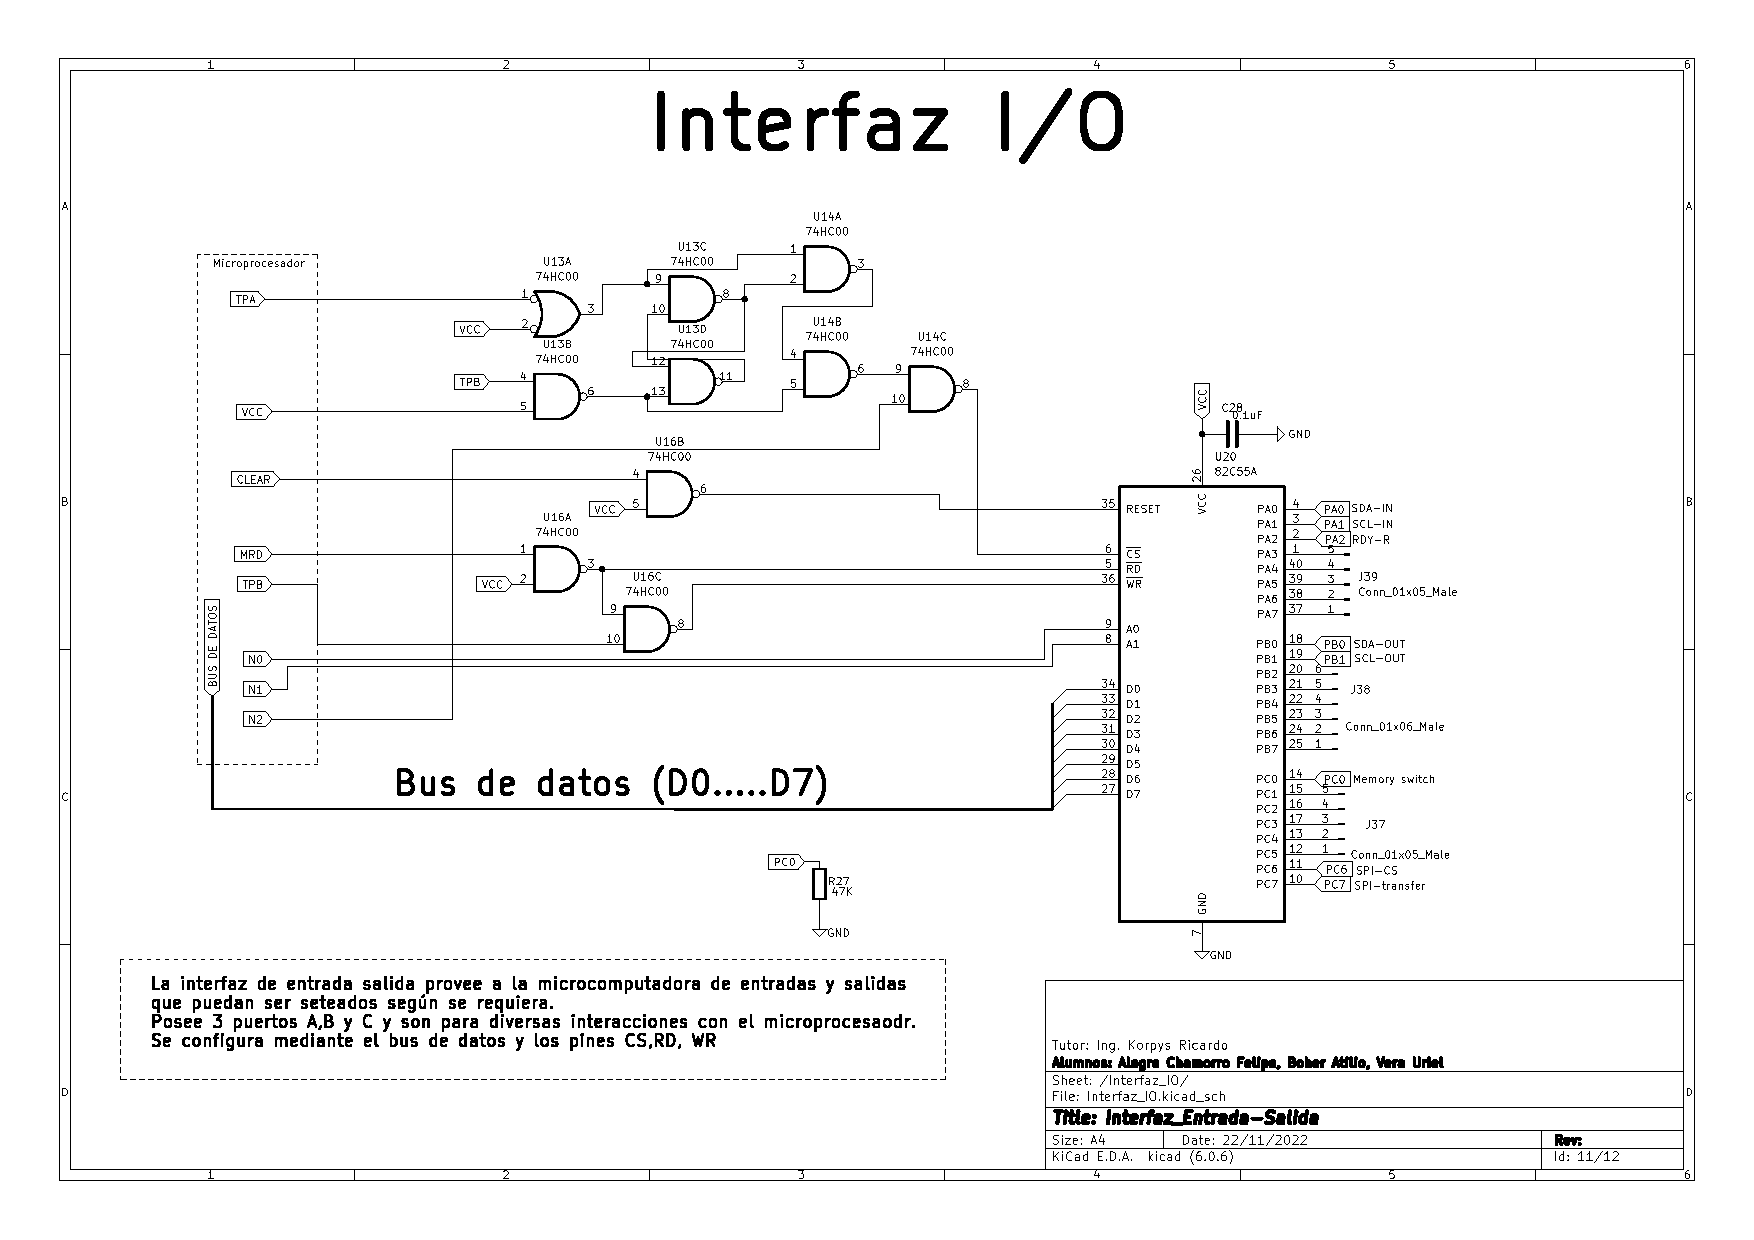
\includegraphics[width=1.2\textwidth, angle=90]{./imagenes/EsquematicosSF/Esquematico (11).pdf}
  \caption{Esquema de interfaz de entrada/salida de sistema final}
  \label{F:EsqSF11}
\end{figure}

Con este circuito es posible controlar las salidas y leer las entradas del 82C55 utilizando las instrucciones de entrada y salida del CDP1802 (INP y OUT). Todas las instrucciones utilizables se encuentran en las tablas~\ref{T:82c55_inp} y \ref{T:82c55_out}, junto a una descripción de la acción realizada por las mismas.

\begin{table}[ht!]
\caption{Instrucciones INP utilizables con el 82C55}
\label{T:82c55_inp}
\begin{tabular}{|c|c|}
\hline
Instrucción & Acción \\ \hline \hline
INP 4       & Guarda en M(R(X)) y en D el dato presente en el puerto A del 82C55     \\ \hline
INP 5       & Guarda en M(R(X)) y en D el dato presente en el puerto B del 82C55    \\ \hline
INP 6       & Guarda en M(R(X)) y en D el dato presente en el puerto C del 82C55    \\ \hline
INP 7       & Guarda en M(R(X)) y en D el dato presente en el registro de control del 82C55     \\ \hline
\end{tabular}
\end{table}

\begin{table}[ht!]
\caption{Instrucciones OUT utilizables con el 82C55}
\label{T:82c55_out}
\begin{tabular}{|c|c|}
\hline
Instrucción & Acción \\ \hline \hline
OUT 4       & Escribe el dato M(R(X)) en el puerto A del 82C55     \\ \hline
OUT 5       & Escribe el dato M(R(X)) en el puerto B del 82C55     \\ \hline
OUT 6       & Escribe el dato M(R(X)) en el puerto C del 82C55     \\ \hline
OUT 7       & Escribe el dato M(R(X)) en el registro de control del 82C55     \\ \hline
\end{tabular}
\end{table}

\clearpage
\subsection{BUS I2C}
\label{C:BUSI2C}

El esquema presentado para el bus I2C presenta una interfaz construida a partir de transistores NPN. La razón de esta interfaz radica en la característica de los dispositivos I2C, que se conectan al bus mediante una interfaz de drenador abierto. Esto podría generar cortocircuitos en un accionamiento simultáneo del bus, por lo que se requiere de esta interfaz.

\begin{figure}[ht]
  \centering
  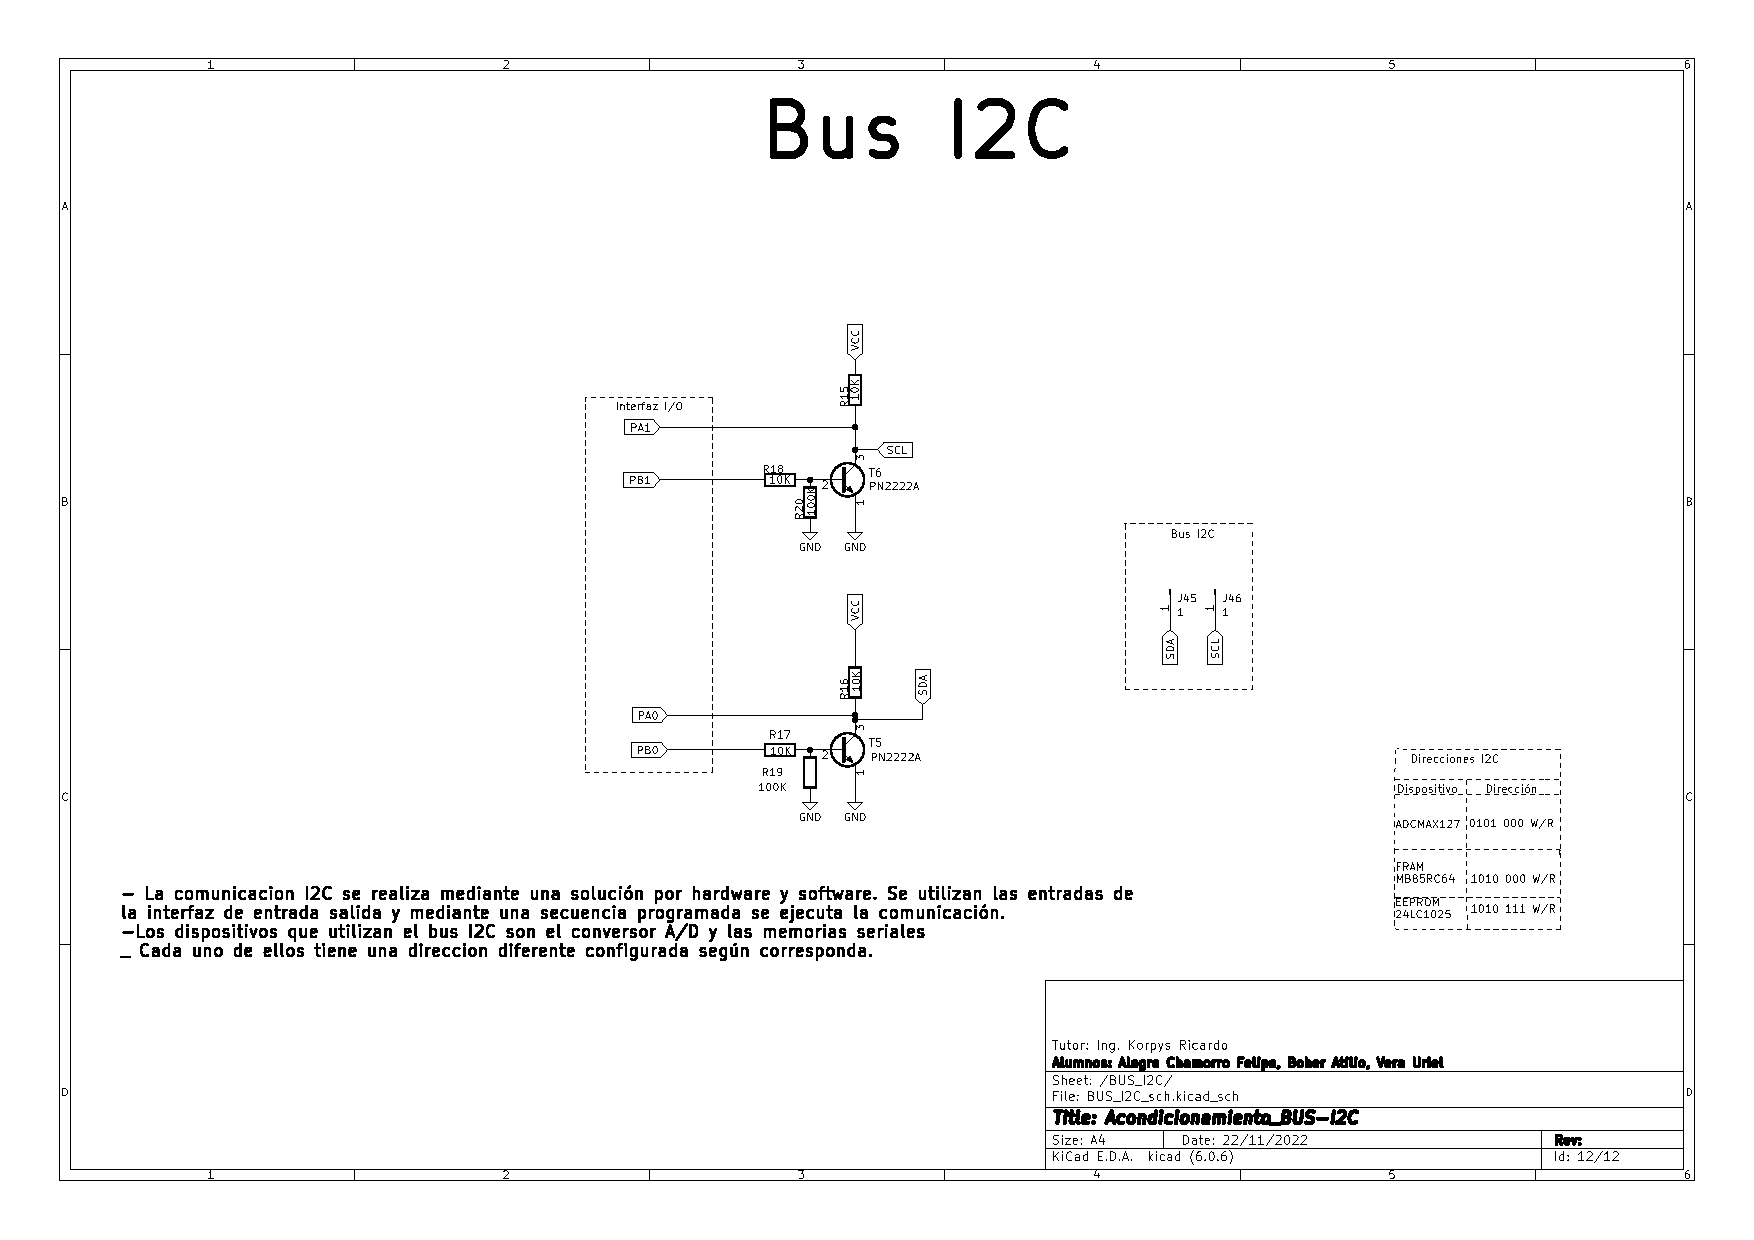
\includegraphics[width=1.2\textwidth, angle=90]{./imagenes/EsquematicosSF/Esquematico (12).pdf}
  \caption{Esquema de bus I2C de sistema final}
  \label{F:EsqSF12}
\end{figure}

\clearpage
\section{Lista de componentes}

En la tabla~\ref{T:bom_sis_final} se encuentra la lista de materiales para la construcción del sistema final.

\footnotesize
\begin{longtable}{|p{0.08\textwidth}|p{0.11\textwidth}|p{0.30\textwidth}|p{0.14\textwidth}|p{0.15\textwidth}|}
\caption{Lista de componentes del sistema final} % needs to go inside longtable environment
\label{T:bom_sis_final}
\\
\hline
Cantidad & Etiqueta \newline
           Identificador            & Descripción                               & Fabricante            & Número de parte       \\ \hline \hline \endfirsthead
\hline
Cantidad & Etiqueta \newline
           Identificador            & Descripción                               & Fabricante            & Número de parte       \\ \hline \hline \endhead
1       & U1                        & Microprocesador                           & RCA                   & CDP1802ACE            \\ \hline
1       & U2                        & Latch de 8 bits                           & Philips               & 74HC573N              \\ \hline
1       & U3                        & Memoria EEPROM 32k x 8                    & XICOR                 & X28C256D-25           \\ \hline
1       & U4                        & Memoria EEPROM Serial I2C 128k x 8        & Microchip             & 24LC1025              \\ \hline
1       & U5                        & Time keeping RAM 32K x8                   & Dallas                & DS1744-070            \\ \hline
1       & U6                        & Memoria RAM 32k x 8                       & HYUNDAI               & HY62256ALP-10         \\ \hline
1       & U7                        & Memoria FRAM Serial I2C 8k x 8            & Fujitsu Semiconductor & MB85RC64A            \\ \hline
1       & U8                        & Conversor analógico-digital con interfaz I2C & Maxim Integrated   & MAX127                \\ \hline
1       & U9                        & Regulador de tensión 12~\si{\volt}        & Motorola              & 7812CT                \\ \hline
1       & U10                       & Regulador de tensión 5~\si{\volt}         & ST Microelectronics   & L7805CV               \\ \hline
1       & U11                       & High Precision Operational Amplifier      & Burr-Brown            & OPA4277PA             \\ \hline
1       & U12                       & Regulador de tensión -12~\si{\volt}       & ST Microelectronics   & L7912CV               \\ \hline
5       & U13, U14, U15, U16, U28   & Cuádruple compuerta NAND de dos entradas  & Texas Instruments     & SN74HC00N             \\ \hline
1       & U17                       & Cuádruple compuerta NAND de dos entradas con Schmitt-Trigger & Texas Instruments& SN74HC132N \\ \hline
2       & U18,U30                   & Cuádruple compuerta NOR de dos entradas   & Texas Instruments     & SN74HC02N             \\ \hline
1       & U19                       & Decodificador Multiplexador 3 a 8 líneas  & Texas Instruments     & SN74HC138N            \\ \hline
1       & U20                       & CMOS Programmable Peripheral Interface    & Intersil              & CP82C55A-5Z           \\ \hline
1       & U21                       & Regulador programable shunt               & Fairchild             & LM336Z25              \\ \hline
1       & U24                       & Doble flip-flop tipo D con Set y Reset    & Texas Instruments     & SN74HC74N             \\ \hline
1       & U25                       & Contador binario de 4 bits                & Fairchild Semiconductor & MM74HC161N          \\ \hline
1       & U29                       & Doble flip-flop JK con Set y Reset        & National Semiconductor & MM74HC73N           \\ \hline
1       & U31                       & Registro de desplazamiento de 8 bits      & Texas Instruments     & SN74HC595N            \\ \hline
1       & U32                       & Registro de desplazamiento de 8 estados   & Motorola              & MC14014BCP            \\ \hline
1       & X2                        & XO-22BE-4MHz                              &   \listaVacio                    & \listaVacio                      \\ \hline
1       & XTAL1                     & Cristal \num{4}~\si{\mega\hertz}          & CQ Electronics        & \listaVacio                      \\ \hline
1       & SW1                       & Llave DPDT 6 pines                        & \listaVacio                      & \listaVacio                      \\ \hline
3       & SW2, SW3, SW4             & Pulsador 6mm~x~4,3mm                      &  \listaVacio                     &  \listaVacio                     \\ \hline
5       & T2, T3, T4, T5, T6        & Transistor BJT NPN                        & Motorola              & P2N2222A               \\ \hline
1       & RV1                       & Preset 10~\si{\kilo\ohm}                  &  \listaVacio                     &  \listaVacio                     \\ \hline
1       & D1                        & Puente rectificador de onda completa B380R &            \listaVacio           &  \listaVacio                     \\ \hline
6       & D2, D3, D4, D5, D6, D7    & LED 5~mm                                  &\listaVacio                       &   \listaVacio                    \\ \hline
2       & D8, D9                    & 1N914                                     &\listaVacio                       &  \listaVacio                     \\ \hline
1       & F1                        & Fusible 10~mm 1~\si{\ampere}              &\listaVacio                       &  \listaVacio                     \\ \hline
8       & R1, R2, R3, R5, R21, R22, R23, R27
                                    & Resistor 47~\si{\kilo\ohm} 1/8~\si{\watt} & \listaVacio                      &   \listaVacio                    \\ \hline
1       & R4                        & Resistor 10~\si{\mega\ohm} 1/8~\si{\watt} &  \listaVacio                     &   \listaVacio                    \\ \hline
1       & R6                        & Resistor 330~\si{\ohm} 1/4~\si{\watt}     &  \listaVacio                     &   \listaVacio                    \\ \hline
2       & R7, R8                    & Resistor 1~\si{\kilo\ohm} 1/8~\si{\watt}  &  \listaVacio                     &    \listaVacio                   \\ \hline
3       & R9, R10, R11              & Resistor 220~\si{\ohm} 1/4~\si{\watt}     &    \listaVacio                   &    \listaVacio                   \\ \hline
16      & R12, R13, R14, R15, R16, R17, R18, R38, R39, R40, R41, R46, R47, R56, R57, R60
                                    & Resistor 10~\si{\kilo\ohm} 1/8~\si{\watt} & \listaVacio                      &   \listaVacio                    \\ \hline
5       & R19, R20, R24, R25, R26   & Resistor 100~\si{\kilo\ohm} 1/8~\si{\watt}&  \listaVacio                     &   \listaVacio                    \\ \hline
4       & R28, R30, R36, R52        & Resistor 100~\si{\ohm} 1/4~\si{\watt}     &  \listaVacio                     &   \listaVacio                    \\ \hline
4       & R29, R31, R37, R53        & Resistor 150~\si{\ohm} 1/4~\si{\watt}     &  \listaVacio                     &   \listaVacio                    \\ \hline
8       & R32, R33, R34, R35, R42, R43, R54, R55
                                    & Resistor 390~\si{\kilo\ohm} 1/8~\si{\watt}&  \listaVacio                     & \listaVacio                      \\ \hline
8       & R44, R45, R48, R49, R50, R51, R58, R59
                                    & Resistor 1~\si{\mega\ohm} 1/8~\si{\watt}  &  \listaVacio                     & \listaVacio                      \\ \hline
2       & C2, C3                    & Capacitor cerámico \num{30}~\si{\pico\farad} 50~\si{\volt}
                                                                                &   \listaVacio                    & \listaVacio                      \\ \hline
14       & C5, C7, C8, C29, C30, C31, C14, C15, C18, C32, C33, C39, C40, C43
                                    & Capacitor cerámico \num{0.10}~\si{\micro\farad} 50~\si{\volt}
                                                                                &    \listaVacio                   &   \listaVacio                    \\ \hline
2       & C11, C17                  & Capacitor electrolítico 4700~\si{\micro\farad} 25~\si{\volt}
                                                                                &     \listaVacio                  &   \listaVacio                    \\ \hline
2       & C12, C16                  & Capacitor cerámico \num{0.33}~\si{\micro\farad} 50~\si{\volt}
                                                                                &   \listaVacio                    &  \listaVacio                     \\ \hline
1       & C13                       & Capacitor electrolítico 10~\si{\micro\farad} 25~\si{\volt}
                                                                                &   \listaVacio                    &  \listaVacio                     \\ \hline
1       & C19                       & Capacitor electrolítico \num{0.01}~\si{\micro\farad} 25~\si{\volt}
                                                                                &     \listaVacio                  &  \listaVacio                     \\ \hline
1       & C20                       & Capacitor electrolítico \num{4.7}~\si{\micro\farad} 25~\si{\volt}
                                                                                &   \listaVacio                    &  \listaVacio                     \\ \hline
6       & J1, J2, J33, J48, J49, J50& 1x3 Pines Conectores Macho \num{2.54}~mm  &   \listaVacio                    &  \listaVacio                     \\ \hline
38      & J3, J4, J5, J6, J7, J8, J9, J10, J11, J12, J13, J14, J15, J16, J17, J18, J19, J20, J21, J22, J23, J24, J25, J26, J27, J28, J29, J30, J31, J36, J40, J41, J42, J45, J46, J51, J52, J53
                                    & Pin conector macho (1 \textit{Male Header Pin}) & \listaVacio                      &   \listaVacio                    \\ \hline
3       & J32, J35, J38             & 1x6 Pines Conectores Macho \num{2.54}~mm  & \listaVacio                      & \listaVacio                      \\ \hline
3       & J34, J37, J39             & 1x5 Pines Conectores Macho \num{2.54}~mm  & \listaVacio                      &   \listaVacio                    \\ \hline
2       & J43, J44                  & Bornera 3 pines \num{5.08}~mm             &  \listaVacio                     &  \listaVacio                     \\ \hline
2       & J47, J54                  & 1x12 Pines Conectores Macho \num{2.54}~mm &   \listaVacio                    &  \listaVacio                     \\ \hline
1       & J55                       & 1x2 Pines Conectores Macho \num{2.54}~mm  &   \listaVacio                    &   \listaVacio                    \\ \hline
1       & No aplica                 & Módulo conversor USB-Serial               & Future Technology Devices International & FT232RL \\ \hline
1       & No aplica                 & Módulo adaptador tarjeta micro SD         & \listaVacio  & \listaVacio \\ \hline
\end{longtable}
\normalsize

\section{Placa PCB}
La placa PCB fue desarrollada en KiCad, al igual que los anteriormente mencionados. En la misma se incluyen todas las partes presentadas en los esquemáticos de la sección \ref{C:EsqSF}. Para ello se requirió un tamaño de 30~cm de largo por 30~cm de ancho, en una placa doble faz. Ambos lados y la máscara de componentes se presentan en las figuras \ref{F:PCB_frente}, \ref{F:PCB_atras} y \ref{F:PCB_mascara}. Sin embargo, se adjuntarán en tamaño original en el apéndice. 
Por otro lado, se presenta una visión en tres dimensiones creada por el mismo software de diseño en la figura~\ref{F:PCB_3D}.


\begin{figure}[H]
  \centering
  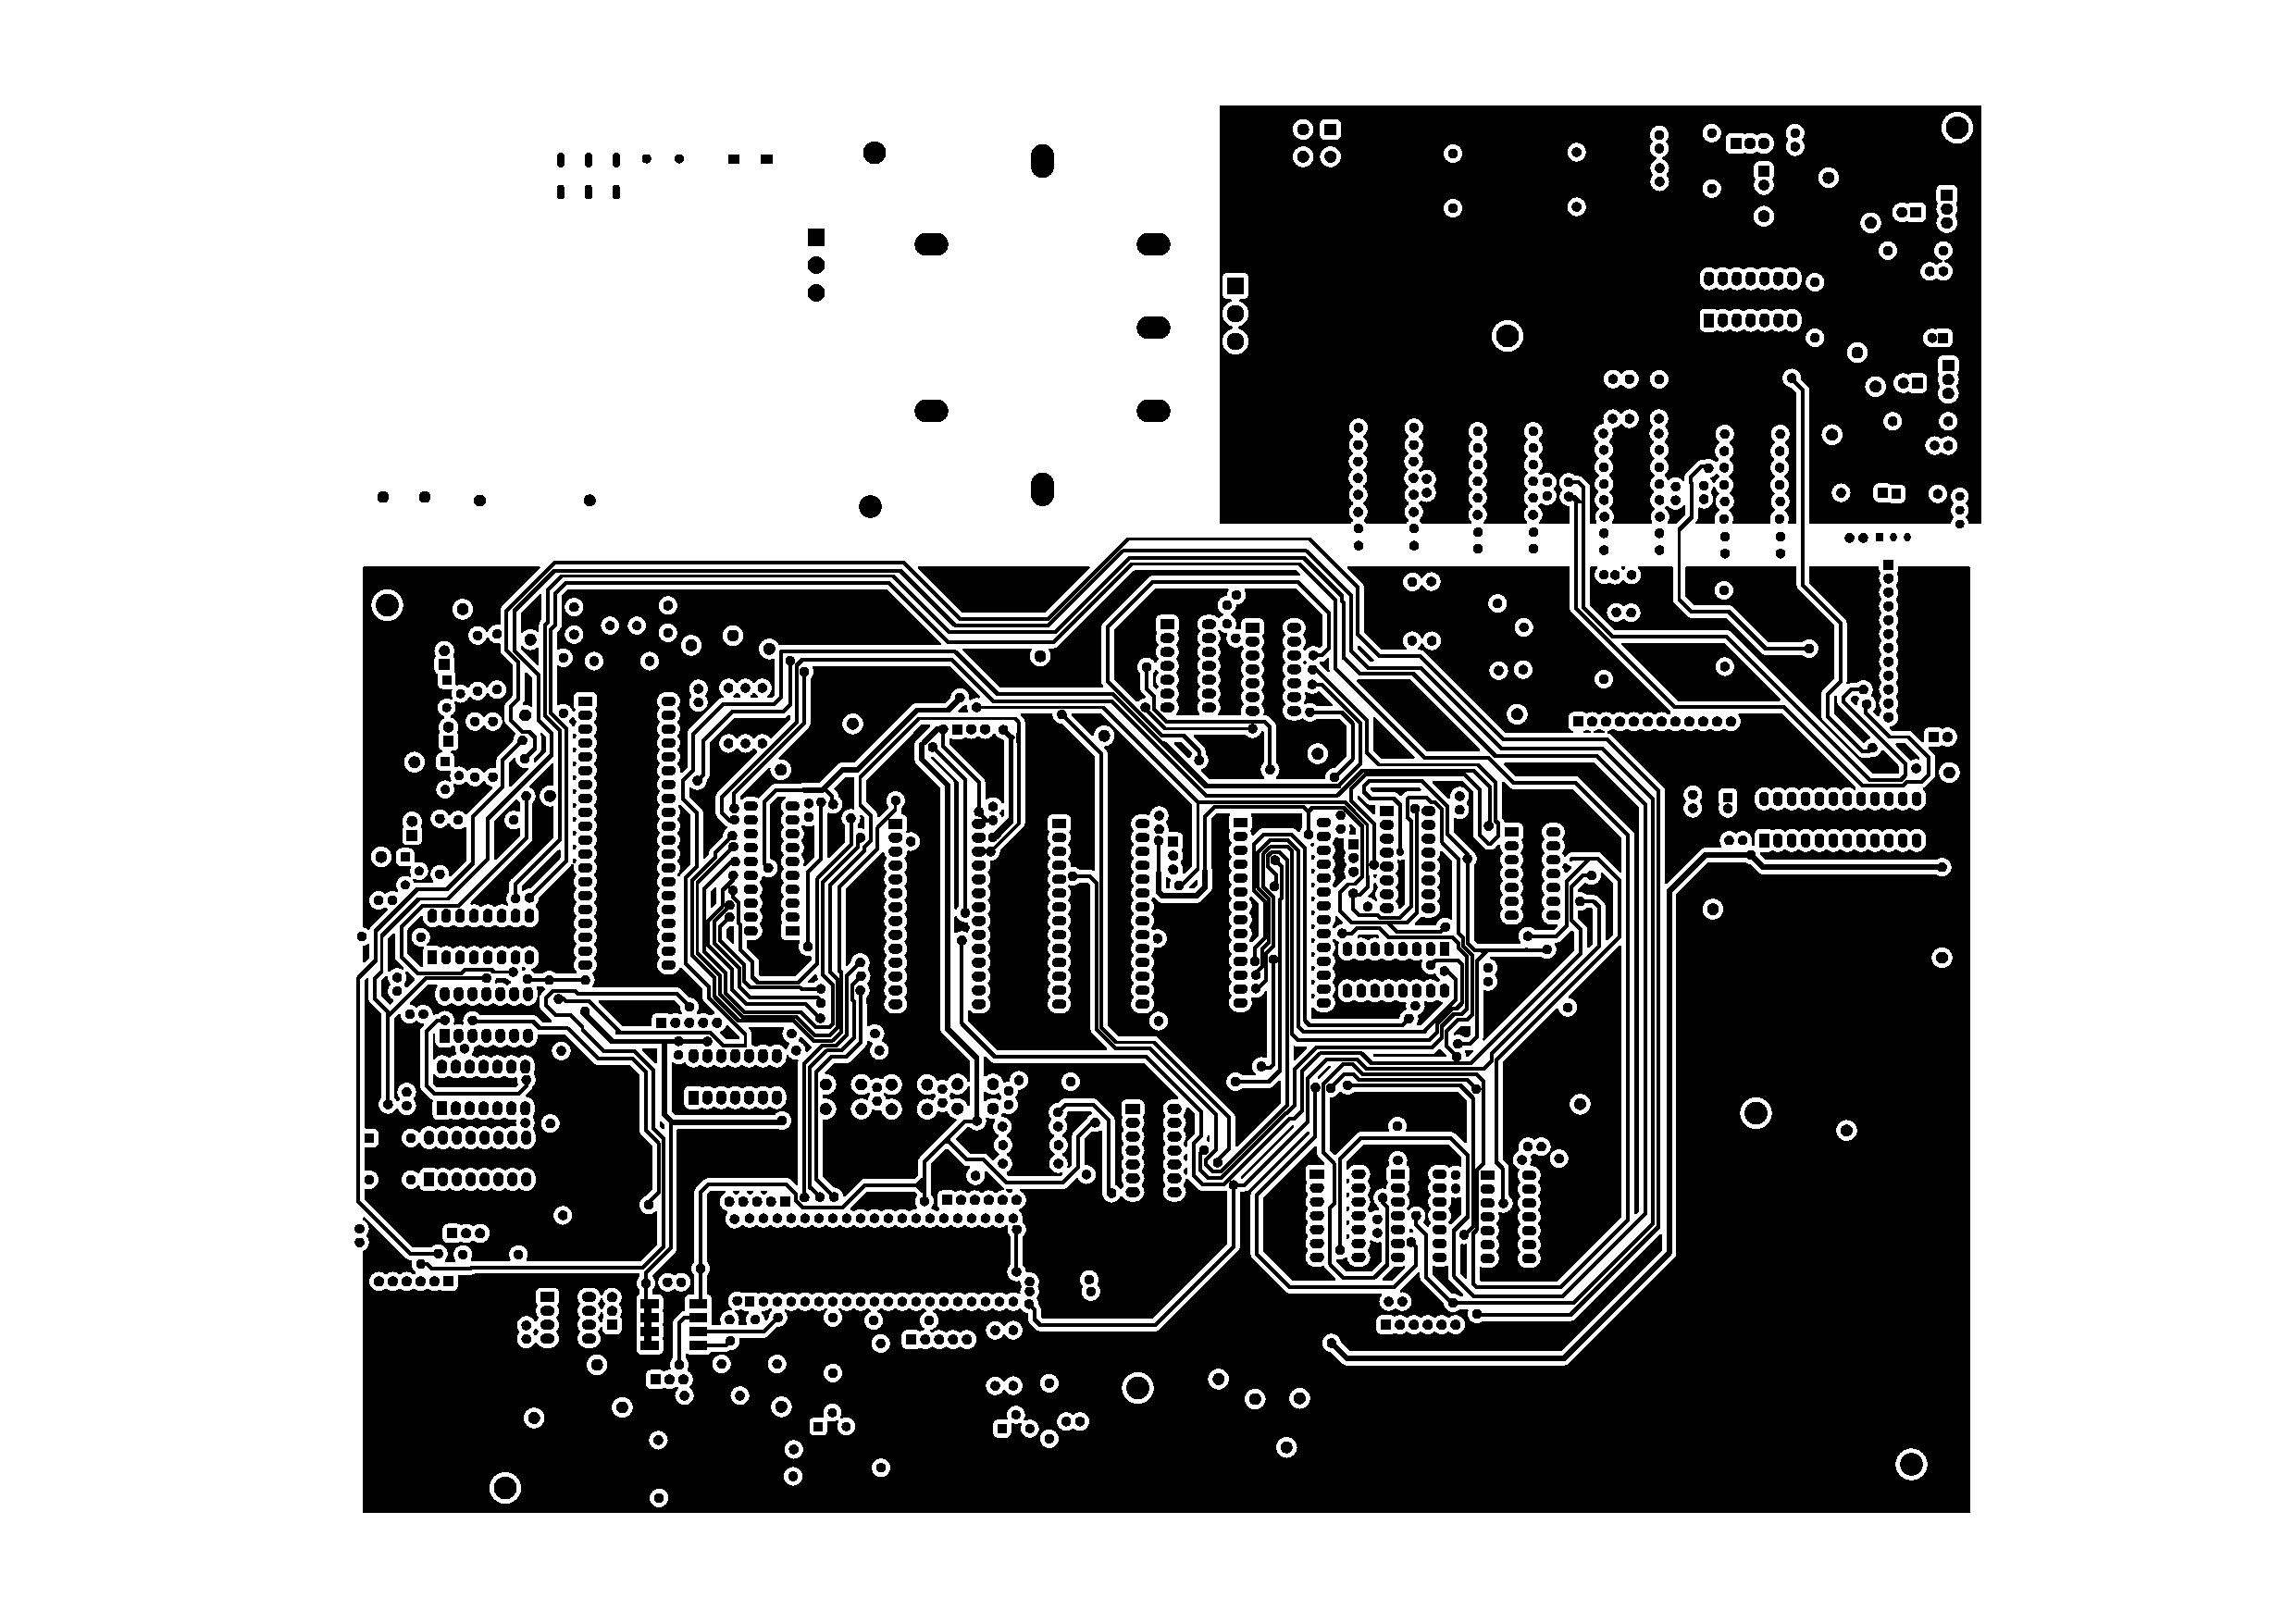
\includegraphics[width=1\textwidth]{./imagenes/EsquematicosSF/PCB_frente.pdf}
  \caption{Pistas de PCB sistema final parte frontal}
  \label{F:PCB_frente}
\end{figure}

\begin{figure}[H]
  \centering
  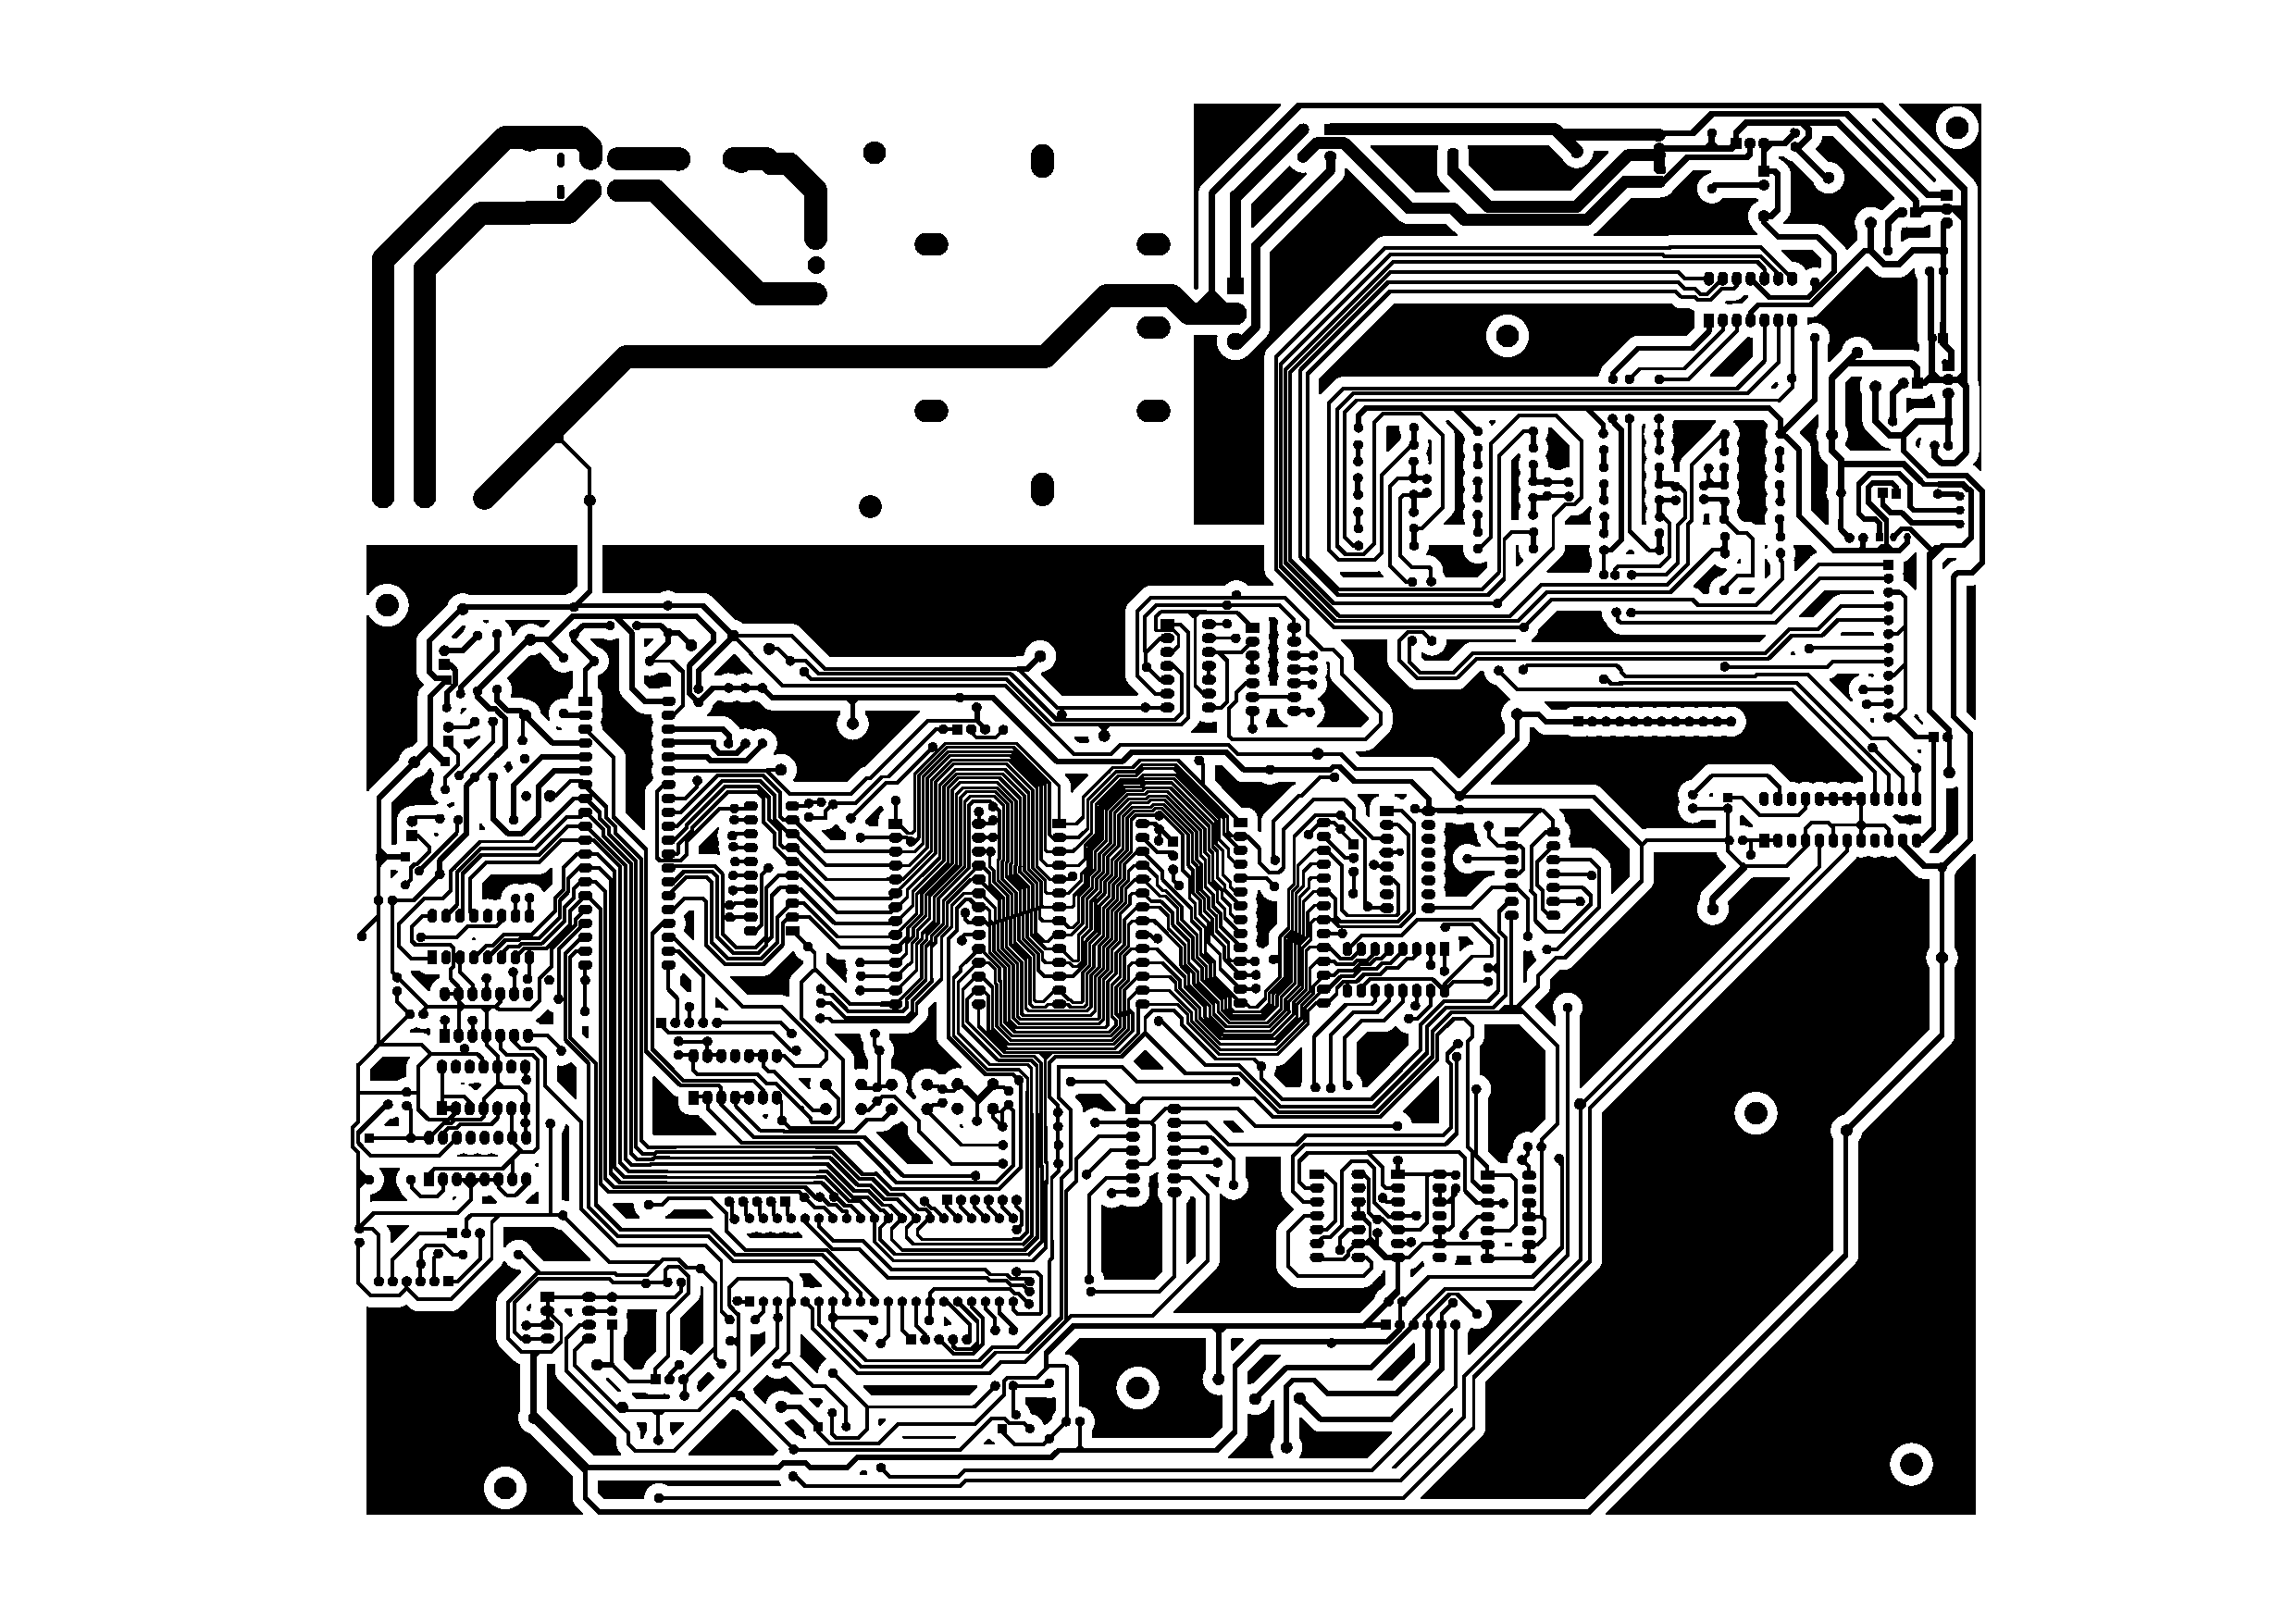
\includegraphics[width=1\textwidth]{./imagenes/EsquematicosSF/PCB_atras.pdf}
  \caption{Pistas de PCB sistema final parte posterior}
  \label{F:PCB_atras}
\end{figure}

\begin{figure}[H]
  \centering
  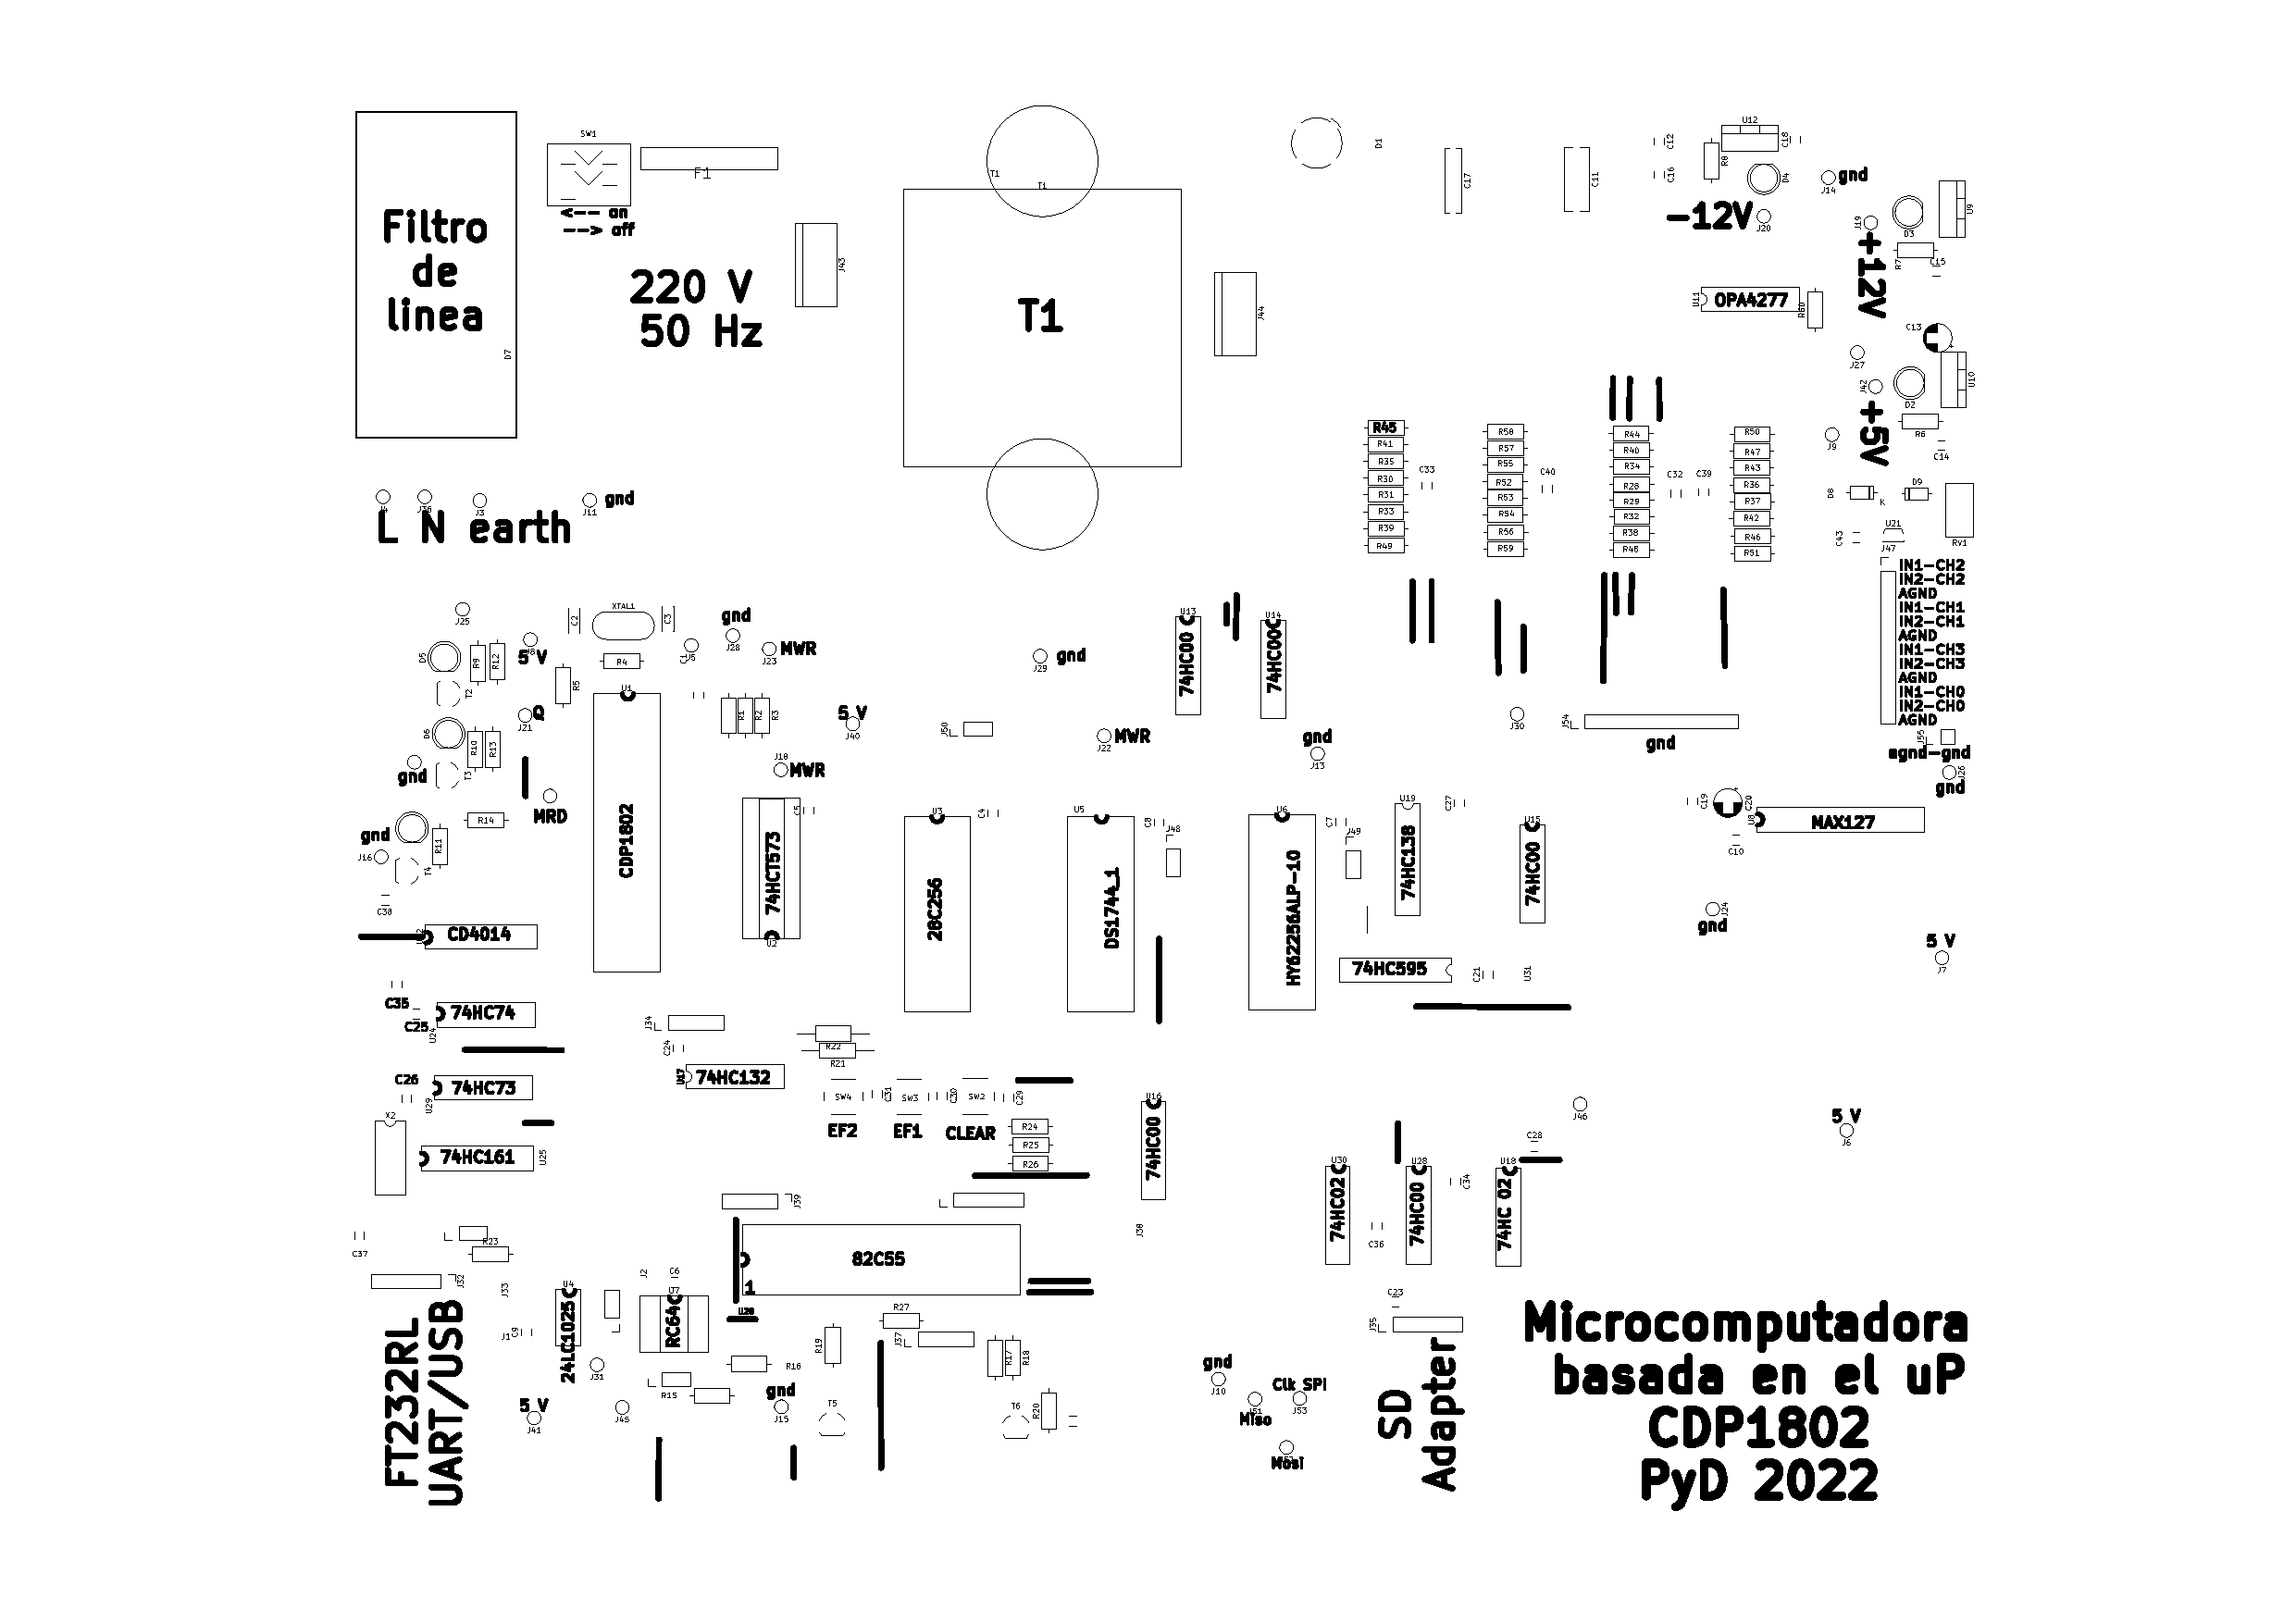
\includegraphics[width=1\textwidth]{./imagenes/EsquematicosSF/PCB_mascara.pdf}
  \caption{Máscara de componentes de PCB de sistema final}
  \label{F:PCB_mascara}
\end{figure}

\begin{figure}[H]
  \centering
  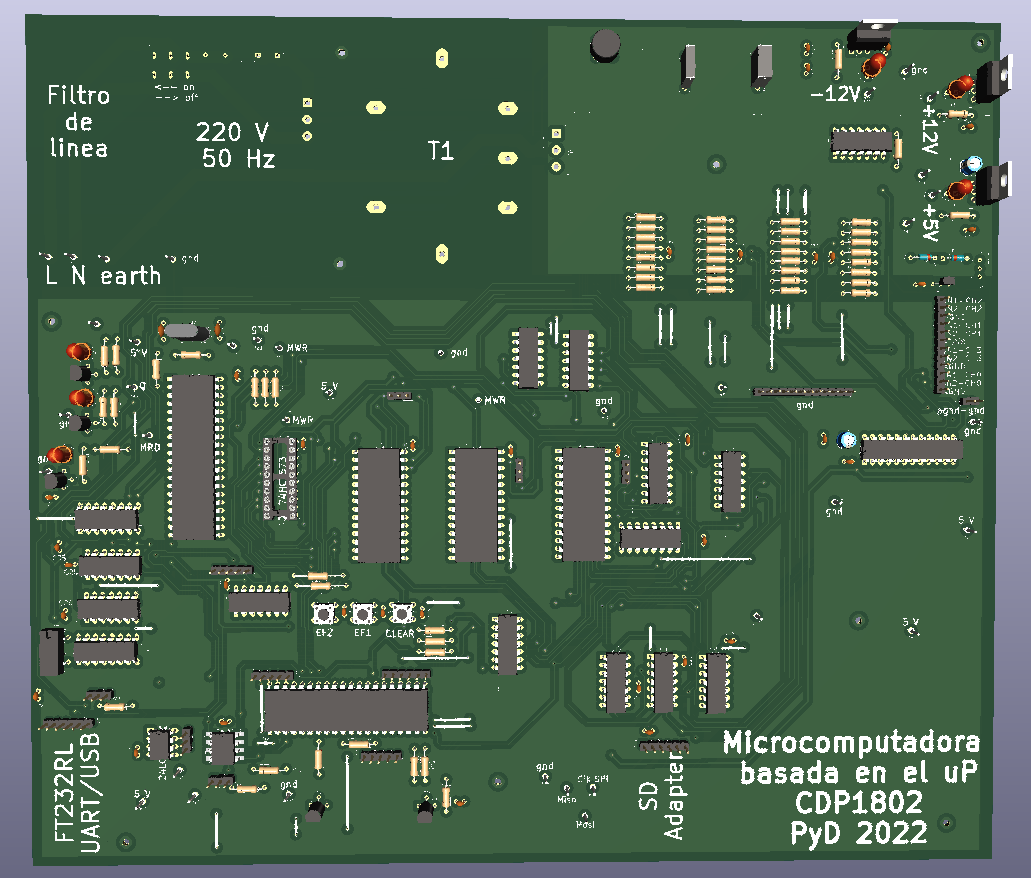
\includegraphics[width=1\textwidth]{./imagenes/sistema_final_3D.png}
  \caption{Visión en tres dimensiones de sistema final}
  \label{F:PCB_3D}
\end{figure}

